% Couverture
\MakeUGthesePDG

\clearpage
\ifodd\value{page}\hbox{}\newpage\fi

\begin{center}\textbf{\large Étude et amélioration de l'exploitation des architectures NUMA à travers des supports exécutifs}

\quad

\textbf{Résumé}
\end{center}

L'évolution du calcul haute performance est aujourd'hui dirigée par les besoins des applications de simulation numérique.
Ces applications sont exécutées sur des supercalculateurs qui peuvent proposer plusieurs milliers de coeurs, et qui sont découpés en un très grand nombre de noeuds de calcul ayant eux un nombre de coeurs beaucoup plus faible.
Chacun de ces noeuds de calcul repose sur une architecture à mémoire partagée, dont la mémoire est découpée en plusieurs blocs physiques différents : cela implique un temps d'accès dépendant à la fois de la donnée accédée ainsi que du processeur y accédant.
On appelle ce genre d'architectures NUMA (pour \emph{Non Uniform Memory Access}).

La manière actuelle de les exploiter tend vers l'utilisation d'un modèle de programmation à base de tâches, qui permet de traiter des programmes irréguliers au dela du simple parallélisme de boucle.
L'exploitation efficace des machines NUMA est critique pour l'amélioration globale des performances des supercalculateurs.
Cette thèse a été axée sur l'amélioration des standards techniques pour leur exploitation : elle propose une réponse au compromis qu'il faut faire entre localité des données et équilibrage de charge, qui sont deux points critiques dans l'ordonnancement d'applications.
Les contributions de cette thèse peuvent se découper en deux parties : une partie dédiée à fournir au programmeur les moyens de comprendre, analyser, et mieux spécifier le comportement des parties critiques de son application, et une autre partie dédiée à différentes améliorations du programme chargé d'exécuter les applications : le support exécutif.
Cette seconde partie a été évaluée sur différentes applications, ce qui a permi de montrer des gains de performances significatifs.



\quad

\textbf{Mots-clés} : trucs

\begin{center}\textbf{\large TODO }

\quad

\textbf{Abstract}
\end{center}

TODO

\quad

\textbf{Keywords} : stuff

%\begin{savequote}[8cm]
%<< Une thèse sans théorème ce n'est pas une thèse >>
%\qauthor{Denis Trystram}
%\end{savequote}
%% Remerciements...
%\chapter*{Remerciements}

%\begin{todo}
%Test todo
%\end{todo}


% TOC
\cleardoublepage
\dominitoc
\makeatletter
\renewcommand{\tableofcontents}[1][\contentsname]{%
  \chapter*{#1}
  \@starttoc{toc}
}
\makeatother
\tableofcontents

\begin{savequote}[6cm]
<< What do you work on?  >>
\qauthor{someone}
\end{savequote}
\chapter{Introduction}
\chaptertoc

L'évolution du calcul haute performance est aujourd'hui dirigée par les besoins des applications de simulation numérique.
Ces applications sont omniprésentes dans l'industrie, et concerne parfois même directement le grand public.

Par exemple des secteurs comme l'aéronautique, les applications militaires, ou encore le nucléaire ont besoin de simuler des phénomènes à grande échelle, se traduisant parfois par la résolution de systèmes de systèmes linéaires à plusieurs millions d'inconnues.
Les prévisions météorologiques à destination du grand public sont faites à l'aide d'applications simulant les intéractions entre les différents éléments de l'atmosphère.
Il en va de même pour tout ce qui se rapporte à l'étude de la propagation des ondes sismiques dans le sol, ou de la prévision de l'impact d'un séisme sur un bassin de population.

Toutes ces simulations sont au final exécutées sur des supercalculateurs, et il n'y a pas de limite aux nombres de ressources qu'elle peuvent utiliser : que ce soit pour améliorer la précision de la simulation, ou augmenter la taille de l'ensemble simulé, elles pourront toujours bénéficier d'un plus grand nombres de ressources.
De plus un grand nombre de ressources peut également permettre d'exécuter un plus grand nombre de simulations simultanément, voire de les coupler entre elles.

Si les supercalculateurs peuvent proposer plusieurs milliers de coeurs, ils sont en fait composés d'un grand nombre de noeuds de calcul avec un nombre de coeurs beaucoup plus faible.
Ces machines peuvent proposer, en plus de processeurs traditionnels, accélérateurs plus ou moins spécifiques comme des GPUs ou des FPGA, formant une architecture dite \emph{hétérogène}.
La très grande majorité des noeuds de calcul intègrent plusieurs processeurs qui accèdent à une mémoire commune.

Contrairement aux processeurs du siècle dernier pour lesquels un changement de génération s'accompagnait d'une augmentation de leur fréquence de fonctionnement, l'évolution des processeurs contemporains se traduit aujourd'hui par la multiplication du nombres de coeurs de calcul qu'ils embarquent.
Pour illustrer ce phénomène il suffit de regarder par exemple la gamme de produits proposés par Intel : la première génération de Pentium 4 - Willamette - lancée par Intel en 2000 était constituée d'un unique coeur cadencé à 1.5GHz. 6 ans plus tard, la dernière génération de Pentium 4 - Cedar Mill - était également consituée d'un seul coeur, mais cette fois cadencé à 3.6 GHz. 10 ans plus tard en 2016, les processeurs de la génération Skylake d'Intel i7 ne dépassent pas les 3.4GHz de fréquence, mais tous ont 4 coeurs physiques au lieu d'un seul.

Avec ce changement de design, les modalités d'accès à la mémoire ont été repensées pour éviter les goulots d'étranglement se formant lors des accès concurrents de plusieurs coeurs au même bus mémoire. Le moyen qui a été trouvé pour éviter trop de contention sur le bus mémoire fut de diviser la mémoire en plusieurs bloc physique différents, avec chacun leur contrôleur.
La conséquence directe de ce changement est que le temps d'accès à la mémoire est devenu non uniforme : il dépend directement de quel processeur essaye d'accéder à quelle partie de la mémoire.
On appelle ce genre d'architectures NUMA (pour \emph{Non Uniform Memory Access}) et elles sont aujourd'hui la brique de base pour créer des supercalculateurs.

L'amélioration des performances générales d'un supercalculateur passe donc directement par l'optimisation de l'exploitation des machines NUMA.
Plusieurs techniques de programmation permette de cibler ce genre d'architectures.
On peut notamment citer des techniques statiques à base de boucles parallèles.
En pratique cela marche particulièrement bien pour les applications où toutes les itérations des boucles sont régulières et où leur temps d'exécution est prévisible.
Néanmoins il existe beaucoup de cas où ce n'est pas le cas.
L'exemple typique est celui des applications de parcours de graphes, qui sont généralement irrégulières.
Mais même dans le cas d'une application où le travail peut sembler régulier, comme par exemple une multiplication de matrices, l'ajout d'une variabilité dans le temps des accès mémoires rend le temps d'exécution difficile à prévoir, et peut entrainer un déséquilibrage de charge.


Les techniques d'ordonnancement dynamiques peuvent garantir une utilisation plus efficace des ressources.
L'une des plus communes est l'ordonnancement par vol de travail : l'application est exprimée comme un graphe de flot de données, chaque sous partie - tâche - consommant et produisant des données.
Un programme dédié - le support exécutif - a la charge d'exécuter ce graphe : à chaque fois qu'un processeur devient inactif, il va récupérer une tâche disponible pour l'exécuter.
Pour que cela soit efficace, il faut pouvoir exprimer un maximum de parallélisme : plus il y a de parallélisme, mieux on est capable d'équilibrer la charge au cours de l'exécution.

Les modèles de programmation standard on su s'adapter : par exemple OpenMP, qui est le standard \emph{de-facto} pour ce genre d'architectures, ne proposait au départ que du parallélisme de boucles. Les dernières versions proposent de la programmation par tâche avec dépendances de données.
En revanche ces modèles de programmation présentent toujours un manque lorsqu'il s'agit d'exploiter efficacement les machines NUMA.
Le programmeur doit donc faire de gros efforts pour effectuer des optimisations spécifiques peu portables, par exemple via des bibliothèques externes pour contrôler précisément le placement des données.
Les outils standard et non intrusifs permettent simplement de distribuer les pages de la mémoire sur les différentes parties physiques : cela a pour avantage d'améliorer l'uniformité des temps d'accès à la mémoire, mais pas d'améliorer le temps d'accès moyen.
Rendant donc les processeurs uniformément mauvais vis à vis de l'accès à la mémoire.

Cette thèse est axée sur l'amélioration des standards et techniques pour l'exploitation des machines NUMA, et cela passe par plusieurs étapes : tout d'abord fournir au programmeur les moyens de comprendre et analyser le comportement des parties critiques de son application.
Ensuite lui permettre de fournir plus d'information au support exécutif, principalement en lui permettant d'exprimer une \emph{affinité} entre ses tâches et les ressources de la machine.
En enfin en proposant des techniques d'ordonnancement prenant en compte ces informations, dans le but d'améliorer efficacement les performances globales de l'application.





\section{Objectifs}\label{sec:intro:objectives}

L'objectif principal de cette thèse était d'étudier les améliorations possibles de l'exploitation des architectures NUMA, à l'aide d'un modèle de programmation à base de tâches.
Cela a été découpé en trois axes de travail.


\subsection*{Analyse du comportement d'applications sur machine NUMA}

Avant de pouvoir penser aux améliorations, il faut commencer par analyser les différents points améliorables, tant du côté logiciel que matériel.
Si l'on souhaitait cibler les modèles de programmation à base de tâches, il fallait néanmoins choisir l'un des modèles existants pour l'étude concrète, et ce choix s'est porté sur OpenMP.

Face à l'absence de suite de benchmarks ciblant certaines fonctionnalités d'OpenMP que nous souhaitions utiliser, nous avons commencé par publier une suite de benchmarks, les KASTORS~\cite{Virouleau2014}.
Les applications présentes dans cette suite ont été adaptées depuis des applications existantes, afin d'utiliser les constructions dont nous avions besoin, et qui sont aujourd'hui utilisées par la communauté.

Nous avons également écrit un outil plus générique, NOMDEL4OUTIL, afin de pouvoir évaluer plus précisément certaines parties ciblées des applications.
L'objectif derrière cet outil est de se libérer de certaines contraintes se présentant lors de l'observation de ces parties de code au cours de l'exécution complète du programme.
En extrayant les parties critiques on peut faire varier à loisir, et précisément, des paramètres tels que le placement des données ou le jeu de données en entrée, afin d'analyser finement quels impacts ils ont et comment l'architecture sous-jacente réagit.


\subsection*{Quelles améliorations pour l'utilisateur et le support exécutif ?}

À partir des conclusions tirées du point précédent, le second objectif était de trouver, proposer, et évaluer des améliorations possibles, tant pour l'utilisateur que pour le support exécutif.

Ces réflexions ont donné lieu à deux contributions : la première est axée sur la réponse au besoin de l'utilisateur, en proposant une clause |affinity| pour les tâches OpenMP~\cite{Virouleau2016b}.
Cette clause a pour but de permettre à l'utilisateur d'indiquer explicitement un lien fort entre une tâche et une ressource de la machine, que ce soit un coeur, un noeud, ou une donnée.
La seconde est axée sur l'extension du support exécutif~\cite{Virouleau2016a}, d'une part pour faciliter la distribution des données sur la machine, et d'autre part pour exploiter les informations disponibles sur les données manipulées par les tâches, dans le but d'améliorer la localité des données au cours de l'exécution.


\subsection*{Place des travaux dans l'évolution du matériel et du logiciel}

Au cours de cette thèse les architectures NUMA ont évolué, on peut alors se demander dans quelle mesure l'évolution du matériel impacte les travaux de cette thèse.
Le dernier objectif est donc d'analyser les travaux effectués - voir les compléter - afin de proposer des approches indépendantes du matériel, dans le but de faciliter le travail du programmeur et du développeur de support exécutif à l'avenir.

Parmi nos travaux, NOMDEL4OUTIL propose une approche transposable à tout type d'architecture, et nous avons fait des travaux préliminaires sur un simulateur, qui à partir des données de cet outil peut donner un aperçu des performances de l'application complète.
Le coût - en temps - de changer l'implémentation utilisée par un support exécutif est assez important, ces travaux préliminaires ont pour objectif de donner un premier aperçu de l'impact que pourrait avoir une modification de l'ordonnancement par le support exécutif.
Cela permet ainsi, lors du "portage" d'une application ou d'un support exécutif sur une nouvelle architecture, d'estimer son comportement, et évaluer si des changements dans l'un des deux sont nécessaires.

\section{Organisation du contenu du manuscrit}\label{sec:intro:outline}

Le manuscrit est découpé en trois grandes parties.
La première partie traite des problématiques abordées par cette thèse, ainsi que des approches existantes sur les points techniques abordés.
Dans cette partie, le chapitre~\ref{chap:contexte} introduit les éléments de base nécessaires au déroulement de cette thèse : les architectures à mémoire partagée, les moyens existants de les programmer, et une description détaillée de certains outils et concepts techniques fondamentaux.
Le chapitre~\ref{chap:rw} revient sur l'état de l'art des techniques utilisées ou étendues par nos travaux.

La seconde partie regroupe nos travaux sur l'étude des machines NUMA, et l'amélioration de leur utilisation à travers OpenMP.
Le chapitre~\ref{chap:contrib:characterization} décrit nos efforts pour étudier le comportement des applications et de l'architecture sous jacente, et décrit l'orientation des travaux à la suite de nos observations.
Les extensions du langage et du support exécutif sont motivées, décrites et évaluées dans le chapitre~\ref{chap:contrib:openmp}.

Enfin la dernière partie se concentre sur les perspectives : le chapitre~\ref{chap:conclusion} revient sur l'évolution du matériel et du logiciel pendant la thèse, et discute des pistes de recherche envisageables pour pousser plus loin nos idées, avant de conclure notre travail et ce manuscrit.



\part{Problématiques impliquées et approches existantes}

\begin{savequote}[6cm]
<< Some great quote  >>
\qauthor{François Broquedis}
\end{savequote}
\chapter{Contexte}\label{chap:contexte}
\chaptertoc

L'objectif de ce chapitre est de donner au lecteur les connaissances de base nécessaires pour l'appréciation du reste de la thèse.

Cela peut se classer en 3 catégories : la première concerne les architectures cibles pour nos travaux. Il y a une grande variété de matériels disponibles pour le calcul haute performance, et la section~\ref{sec:context:numa} décrit en détails les architectures à mémoire partagée actuelles (NUMA).
La seconde concerne les modèles de programmation à base de tâche. La section~\ref{sec:context:others} décrit les techniques modernes utilisées pour cibler les architectures NUMA, et décrit en détails les concepts de base ainsi que les points clés pertinents à nos travaux. La section~\ref{sec:context:openmp} est dédiée à OpenMP, modèle de programmation qui a été utilisé pour l'application des travaux de la thèse.
Enfin la section~\ref{sec:context:runtimes} regroupe des informations générales concernant l'ordonnancement d'applications par des supports exécutifs.

\section{Shared memory architectures}\label{sec:context:numa}



\subsection{Single node design}

Talk about cache hierarchy, maybe give some number and a drawing of how it looks like?

\subsection{Interconnecting nodes}

Talk about how nodes are interconnected with each other, give some numbers (?) and some drawing.

\section{Modèles de programmation à base de tâches}\label{sec:context:others}

Il existe de nombreux modèles de programmation à base de tâches, certaines fonctionnalités diffèrent, mais les concepts de base restent les même, et seront détaillés ci dessous.

\begin{todo}

  -> parler protocole de cohérence de cache (dans interconnexion peut être)
  -> remonter les sections archi, le cache mérite son propre truc
  -> Parler briévement des modèles de programmation exotiques, en disant qu'ils seront abordé en détail en 3
  -> motiver pourquoi cilk, tbb, et openmp (anotation sur fonction, code utilisateur, simple pragma)
\end{todo}

\subsection{L'unité de base : la tâche}

Une tâche peut être vue comme la plus petite quantité de travail séquentiel exécutable sur un processeur.
En pratique c'est une section de code bien définie du programme, et cela peut être une simple instruction, un bloc de code délimité, ou encore une fonction très complexe.
La quantité de calcul idéale dans une tâche - la \emph{granularité} - peut varier fortement en fonction de l'application et du support exécutif, ce point est abordé en détail dans la section~\ref{sec:context:others:granularity}

Une tâche est nécessairement accompagnée de données qu'elle manipule. De la même manière qu'une fonction utilise des paramètres, le bloc de code composant une tâche utilise des variables qui peuvent être soit locales (on parlera alors de données privées), soit partagées par d'autres parties du code (on parlera de données partagées).


\subsection{Traitement d'une tâche : de la création à l'exécution}\label{sec:context:others:costs}

Si la notion de tâche peut paraître simple, elle s'accompagne d'un certain nombre de traitement plus ou moins automatique (en fonction du modèle de programmation), mais qui dans tous les cas a un coût.
Les trois paragraphes suivants décrivent quelques points clés accompagnant l'utilisation des tâches, qui sont parfois cachés au programmeur.

\subsubsection{Création}

En fonction du modèle de programmation, la création d'une tâche peut être plus ou moins pénible pour le programmeur.

Prenons deux exemples représentatifs pour illustrer.

En StarPU natif, voici par exemple comment on pourrait définir et créer une tâche :

\begin{lstlisting}[language=c++,caption=Exemple simple en StarPU,label=lst:context:simple-starpu,basicstyle=\small]
void work() {
  // calcul
}

int main() {
  // ...
  struct starpu_codelet dummy_big_cl =
  {
    // ...
    .cpu_funcs = { work },
  };

  task = starpu_task_create();
  task->cl = &dummy_big_cl;
  starpu_task_submit(task);
}
\end{lstlisting}

On voit ici que l'utilisateur doit d'une part avoir isolé la partie calcul de son code, et d'autre part interagir avec le support exécutif de manière significative pour créer une tâche.

Si on regarde maintenant un exemple simple en OpenMP :

\begin{lstlisting}
void foo()
{
  // ...
  #pragma omp task
  {
    // calcul
  }
  // ...
}
\end{lstlisting}

Cela parait certes moins intrusif et pénible pour le programmeur, mais pour autant cela ne veut pas dire qu'il y a pas moins d'actions effectuées en pratique !
Que se passe-t-il vraiment ?

Le compilateur ne va pas laisser ces éléments tels quels dans l'objet binaire généré~: il va les transformer en un ensemble de fonctions élémentaires imposées par le support exécutif. Cet ensemble de fonctions élémentaires s'appelle l'\emph{ABI} (pour \emph{Abstract Binary Interface}).

Un exemple de ce type en OpenMP va donc entrainer deux transformations importantes par le compilateur :
\begin{itemize}
  \item l'\emph{outlining} de la fonction, qui consiste à externaliser le code de la tâche et son contexte dans une fonction séparée.
  \item la substitution du pragma par un appel au support exécutif.
\end{itemize}

Cela donnera au final un code binaire généré correspondant à un programme de ce type :

\begin{lstlisting}
void outlined(struct Context c)
{
  // unpacking du contexte, recréation des variables locales
  // calcul
}

void foo()
{
  // ...
  struct Context c;
  // capture des variables partagées
  runtime_specific_create_task(outlined, c);
  // ...
}
\end{lstlisting}

\begin{todo}
  Montrer le packing/unpacking ainsi que les appels au runtime (eg: libomp)
\end{todo}

Au final les actions effectuées pour la création d'une tâche sont équivalentes, bien que parfois cachées.


\subsubsection{Gestion}

Une fois que le programmeur a définie sa tâche et l'a soumise au support exécutif, celui ci doit créer et maintenir une structure de données représentant cette tâche.
Celle ci peut être plus ou moins grande en fonction des informations associées à la tâche.

Le support exécutif va utiliser ces informations au cours de l'exécution du programme pour déterminer quelles tâches sont prêtes pour l'exécution.
En pratique cela signifie que ces structures de données vont être placées dans des conteneurs tels que des files ou des piles, et qu'un certain nombre d'opérations seront effectuées dessus (ajout, suppression, parcours).

En conséquence le coût du maintien des informations à propos d'une tâche entre sa création et son exécution dépend du support exécutif et des structures de données qu'il utilise.


\subsubsection{Exécution}

Cette étape est l'un des points où la gestion par tâche dispose d'un gros avantage par rapport à la création individuelle de thread par le programmeur.
Au début de l'exécution de l'application, un certain nombre de cœurs physiques sont utilisables par le support exécutif (cela peut être déduit implicitement par le support exécutif, ou spécifié explicitement par le programmeur).
Lors de son initialisation, le support exécutif va \textbf{créer et attacher} un thread logique par cœur physique, virtualisant ainsi la gestion des cœurs physiques.

Ces threads vont se voir attribuer différents attributs, comme par exemple une structure de données contenant des tâches.
Ils seront des <<travailleurs>> permanents pour le support exécutif, qui leur donnera des tâches à exécuter au fur et à mesure.

Les threads sont donc les même tout au long de l'exécution de l'application, ce qui évite les coûts liés à la création ou à la destruction de threads. 


\subsection{Moyens de synchronisation}

Lorsqu'on parle de programmation parallèle, il faut bien évidemment parler de synchronisation.
Les différentes tâches définies par l'utilisateur vont être exécutées en parallèle sur la machine, mais dans beaucoup de cas certaines tâches doivent attendre la complétion d'une ou plusieurs tâches avant de pouvoir commencer à être exécutée.

Il y a deux grand types de synchronisations pour la programmation à base de tâche~: la synchronisation explicite, et les dépendances de données.

\subsubsection{Synchronisation explicite}

Le programmeur peut ajouter un point de synchronisation explicite dans le code.
Lorsque le thread exécutant la tâche atteint ce point de synchronisation, il se bloque et attend que l'ensemble des tâches qu'il a créé ait été exécuté avant de reprendre son exécution. Dans l'exemple du listing~\ref{lst:context:task-wait}, exprimé en OpenMP, la tâche C sera garantie d'être exécutée \textbf{après} les tâches A et B.

\begin{lstlisting}[caption=Synchronisation dans le thread courant (OpenMP),label=lst:context:task-wait]
void foo() {
  #pragma omp task
  A();
  #pragma omp task
  B();
  #pragma omp taskwait
  #pragma omp task
  C();
}
\end{lstlisting}


\subsubsection{Dépendances de données}

Le programmeur spécifie des dépendances de données, avec des modes, pour chacune des tâches.
Dans l'exemple du listing~\ref{lst:context:task-dep}, la tâche |write_A| possède une dépendance en \emph{écriture} sur la variable |a|, et la tâche |read_A| possède une dépendance en \emph{lecture}.

Étant donné qu'il y a une lecture et une écriture, le principe de cohérence séquentielle impose que les opérations soit ordonnées dans l'ordre où elles ont été créées (ici la tâche en lecture devrait avoir lieu \textbf{après} la tâche en écriture).

Si on regarde le reste du programme, la tâche |B| dispose d'une dépendance en écriture sur |b| et la tâche |C| souhaite lire |a| et |b|.

Étant donné que du point de vue des dépendances les tâches |write_A| et |B| sont indépendantes, elles pourraient très bien être exécutées en même temps, et |B| pourrait terminer son exécution avant même que |read_A| commence la sienne.

En revanche |C| devra forcément être exécutée après |read_A| et |B| puisqu'elle a une dépendance en lecture sur des données écrites par ces deux tâches, et qu'elle a été créée après dans l'ordre séquentiel.


\begin{lstlisting}[caption=Synchronisation via des dépendances (OpenMP),label=lst:context:task-dep]
void foo() {
  int a;
  int b;
  #pragma omp task depend(out: a)
  write_A(&a);
  #pragma omp task depend(in: a)
  read_A(&a);
  #pragma omp task depend(out: b)
  B(&b);
  #pragma omp task depend(in: a, b)
  C(a, b);
}
\end{lstlisting}

\begin{todo}
GRAPHE : 2.2.2 mini schéma dataflow du graphe correspondant au programme écrit.
\end{todo}

Les deux ont des avantages et des inconvénients : la synchronisation dans le thread courant représente très peu d'overhead lors de l'exécution, mais si le travail est légèrement déséquilibré, certains threads pourraient rester inactifs alors que des tâches pourraient être exécutées.
Les dépendances induisent un coût de calcul des tâches prêtes lors de l'exécution, mais maximise l'utilisation des ressources.


\subsection{Quelques exemples de modèles de programmation}

Plusieurs modèles de programmation populaires proposent d'exprimer du parallélisme à base de tâches, parmi lesquels Cilk, TBB, et OpenMP.

Les listings~\ref{lst:context:cilk},~\ref{lst:context:tbb}, et ~\ref{lst:context:openmp} donnent une comparaison de l'expression du même exemple simple, le calcul du nième nombre de la suite de Fibonacci.

\subsubsection{Cilk}

Cilk~\cite{cilk5} est un modèle de programmation basé sur C.
Il introduit principalement deux nouveaux mots clés : |cilk_spawn| et |cilk_sync|, pour, respectivement, exposer du parallélisme et introduire un point de synchronisation.
Le mot clé |cilk_spawn| vient précéder un appel de fonction pour indiquer que la fonction peut s'exécuter en parallèle. Cela en fait donc un modèle de programmation à base de tâches.
Cilk propose également une extension de la notation de tableau, ayant pour but de faciliter la vectorisation automatique par le compilateur.


\begin{lstlisting}[language=c++,caption=Fibonacci exprimé en Cilk,label=lst:context:cilk,basicstyle=\small]
int fib(int n) {
  if (n < 2)
    return n;
  int x = cilk_spawn fib(n-1);
  int y = fib(n-2);
  cilk_sync;
  return x + y;
}
\end{lstlisting}


\subsubsection{Threading Building Block}

Threading Building Block (TBB)~\cite{Reinders2007} est un modèle de programmation développé par Intel comme une bibliothèque C++.

Elle propose différentes fonctions pour que le programmeur puisse exprimer du parallélisme, dont notamment :
\begin{itemize}
  \item La fonction template |parallel_for|, s'appliquant sur une boucle et prenant en paramètre une fonction utilisateur.
    La bibliothèque découpe automatiquement l'espace d'itération en groupes d'itérations et envoie un itérateur C++ à la fonction utilisateur pour son traitement.
  \item Un ensemble de fonctions pour accéder à l'ordonnanceur de tâches de la bibliothèque.
\end{itemize}

La bibliothèque propose également un ensemble de structures de données à accès concurrent (listes, tables de hachage), ainsi que des allocateurs mémoires.

\begin{lstlisting}[language=c++,caption=Fibonacci exprimé en TBB,label=lst:context:tbb,basicstyle=\small]
#include "tbb/task_group.h"
using namespace tbb;

int Fib(int n) {
  if( n<2 ) {
    return n;
  } else {
    int x, y;
    task_group g;
    g.run([&]{x=Fib(n-1);}); // création d'une tâche
    g.run([&]{y=Fib(n-2);}); // création d'une autre tâche
    g.wait();                // synchronisation
    return x+y;
  }
}
\end{lstlisting}

\subsubsection{OpenMP}

OpenMP~\cite{openmp45} est un modèle de programmation supportant le C/C++ et Fortran.
Il s'utilise à travers des directives de compilation ainsi qu'une API, et propose lui aussi les constructions classiques : boucles, tâche, et autres éléments facilitant la programmation parallèle.

Originellement OpenMP ne proposait que du parallélisme de boucle, le concept de tâches n'a été introduit que plus tard avec OpenMP~3.0, et le concept de dépendances de données entre tâches a été introduit encore plus tard avec la version~4.0.

Le standard d'application de nos idées pour cette thèse étant OpenMP, une description détaillée des fonctionnalités et de ses spécificités est faite dans la section~\ref{sec:context:openmp}.

\begin{lstlisting}[language=c++,caption=Fibonacci exprimé en OpenMP,label=lst:context:openmp,basicstyle=\small]
int fib(int n) {
  if (n < 2)
    return n;
#pragma omp task
  int x = fib(n-1);
  int y = fib(n-2);
#pragma omp taskwait
  return x + y;
}
\end{lstlisting}

\subsection{Quantité de travail et granularité}\label{sec:context:others:granularity}


Dans ce type de modèles de programmation, la clé pour maximiser l'utilisation des ressources est de réduire l'overhead du support exécutif par rapport au calcul en trouvant le bon \emph{grain} de tâche.

Il faut donc jouer sur le degré de parallélisme pour atteindre les meilleures performances : les tâches doivent être suffisamment petites pour proposer le maximum de parallélisme, mais pas trop pour ne pas surcharger le support exécutif, vis à vis des coûts décrits dans la section~\ref{sec:context:others:costs}.

Ce grain optimal dépend de plusieurs facteurs : les structures de données utilisées par le support exécutif, le coût de création des tâches, et la quantité de travail mis à disposition par cœur via ce grain.

Cela peut être illustré via une application telle que la factorisation de Cholesky par bloc : à taille de matrice fixée le nombre de tâches créées dépend directement de la taille de bloc choisie.
Plus la taille de bloc est petite, plus le nombre de blocs créés (et donc le nombre de tâches, et le parallélisme potentiel) est important.

\begin{todo}
%\begin{figure}[ht]
	%\centering
	%\includegraphics[width=0.66\textwidth]{todo}
	%\caption{todo}\label{fig:context:granularity}
%\end{figure}
  courbe grain
\end{todo}

La figure~\ref{fib:context:granularity} illustre l'évolution des performances d'une factorisation de Cholesky d'une matrice de taille 8192, sur un nombre de cœurs fixé (64), en fonction de la taille de bloc et du support exécutif.
Comme on peut le voir, les parties extrèmes de la courbe se comportent de manière similaires quelque soit le support exécutif : une taille de bloc trop faible génère beaucoup trop de tâches et les support exécutifs sont complètement surchargés. Une taille de bloc trop importante limite complètement le parallélisme et donc les performances.

Le grain adapté n'est pas nécessairement unique : en fonction du support exécutif on peut avoir un choix plus ou moins important (TODO : mettre les vrais chiffres d'ompss et de libkomp/gcc).

La courbe tracée avec libkomp inclue nos travaux sur l'affinité, et cela permet d'illustrer que même si cela permet d'influer sur les performances maximales, cela a un impact minimal sur le grain.



Le choix du grain pour une tâche dépend entièrement de l'application, et reste à l'appréciation du programmeur.

\subsection*{Conclusion}

Bien que tout ces modèles de programmation aient leur spécificités, ils permettent tous de décrire l'application sous forme de graphe de tâches direct et acyclique (DAG).

L'étape suivante consiste à exécuter ce graphe sur la machine, et pour cela le support exécutif peut se reposer sur un ensemble important de techniques d'ordonnancement. 



\section{Supports exécutifs}\label{sec:rw:other-runtimes}

Il existe un certain nombres d'autres supports exécutifs, pour OpenMP comme d'autres modèle de programmation.
Les sections ci après introduisent ceux ayant des thématiques très proches de cette thèse.

\subsection{XKaapi}

XKaapi~\cite{Gautier2007} est un support exécutif, à base de tâche avec dépendances, ciblant les architectures multicœurs et hétérogènes.
Il repose sur hwloc pour découvrir la topologie de la machine, et utilise ces informations à de multiples endroits.

XKaapi dispose d'un nombre important de fonctionnalités spécifiques à l'ordonnancement de tâches.
Une attention particulière a été portée au coût de création des tâches au sein du support exécutif, qui a été diminué au maximum (TODO : ref needed).
Le moteur d'ordonnancement de XKaapi fonctionne par vol de travail, et implémente les étapes critiques de \emph{sélection} et de \emph{placement} décrites dans la section~\ref{sec:context:runtimes:ws}. Il est facile d'ajouter des heuristiques additionnelles pour ces deux étapes, ce qui nous a permis d'implémenter dans ce support exécutifs les extensions décrites dans la section~\ref{sec:contrib:ws:heuristics}.

Le nombre de files de tâches repose sur les informations fournies par hwloc~: XKaapi implémente une file de tâches par niveau de la hiérarchie (i.e.~: une file par cœur, une file par nœud NUMA, etc...), qui sont éventuellement utilisées par les heuristiques.

Pour la gestion de ces files, XKaapi implémente le protocole THE~\cite{cilk5} proposé par Cilk. Ce protocole permet de faire de manière non bloquante des accès concurrent à la même file de tâche. Le principe est le suivant~: le \emph{voleur} - distant - va venir prendre des tâches en tête de file, et la \emph{victime} (ou le thread local) va venir ajouter ou retirer des tâches en queue de file.
Le seul conflit se produit lorsque la file n'a qu'un seul élément, et il peut être résolu par un simple \emph{compare-and-swap}, se traduisant par un échec de la requête pour l'un, et un succès pour l'autre.

En plus de l'utilisation de ce protocole, XKaapi peut effectuer de l'agrégation de requêtes de vols~: lorsque plusieurs voleur font effectuer des requêtes sur la même victime, seul le premier voleur arrivé va effectuer la requête de vol, et récupérer suffisamment de tâche pour l'ensemble des voleurs.
Les gains théoriques liés à ce mécanismes ont été étudiés par Tchiboukdjian et al.~\cite{Tchiboukdjian2010a}.

Pour observer le comportement des applications exécutées, il dispose d'un outil de génération de traces.
Cela permet une analyse pointue du comportement de l'application, à travers les compteurs de performances matériels et une analyse par type de tâche.
Cet outil nous a permis de faire des observations préliminaires déjà très poussées, sur une étude de cas abordée dans la section~\ref{sec:contribs:apps:cholesky:observations}.

XKaapi est principalement utilisé comme prototype de recherche, et a été utilisé pour l'implémentation de certains travaux proches des thématiques de cette thèse, en particulier celle de la localité des données~\cite{Durand2013, Bleuse2014, Lima2015}.

Enfin il dispose d'une couche de compatibilité pour OpenMP, nommée libKOMP~\cite{Broquedis2012}.
Cette couche implémente à la fois les ABIs de libGOMP et libOMP, ce qui permet de l'utiliser pour exécuter des programmes OpenMP~4.5 directement en compilant via GCC ou Clang, et en changeant le support exécutif chargé à l'exécution.



\subsection{libGOMP}

libGOMP~\cite{Novillo2006} est le support exécutif OpenMP fourni avec le compilateur GCC.

Au niveau des fonctionnalités, il implémente la totalité du standard OpenMP~4.5.
Comme la majorité des supports exécutifs, libGOMP réutilise les threads qui sont créés entre différentes région parallèles successives, pour éviter d'avoir à payer le coût de destruction/création d'un thread inutilement.
Les gestion des constructions à base de boucles et de tâches sont complètement séparées dans le support exécutif.
Vis à vis de la hiérarchie de l'architecture cible, il n'y a aucune disposition particulière pour essayer de la prendre en compte.

Pour la gestion des tâches, il a des différences majeures dans la manière de fonctionner par rapport à XKaapi~: il fonctionne bien par vol de travail, mais en revanche il n'y a qu'une seule file de tâches par \emph{team}, et donc une seule file pour l'ensemble des threads !
Si fonctionnellemment cette caractéristiques n'est pas un problème, cela peut avoir un impact sur les performances compte tenu du fait que tous les threads devront se synchroniser pour accéder à la même struture de données.
Cela se voit d'ailleurs sur la figure~\ref{fig:context:granularity} illustrant l'impact de la granularité des tâches~: pour des petites tailles de bloc (et donc un grand nombre de tâches), libGOMP est loin derrière à cause du surcout entrainé par la gestion de la liste de tâches.
(cf figure 2.4 sur la granularité)

Néanmoins, en tant que support exécutif grand public et largement utilisé, il constitue une référence intéressante.

\subsection{libOMP}

libOMP est le support exécutif OpenMP fourni avec le compilateur Clang, directement basé sur le support exécutif d'Intel fourni avec ICC.
Ils partagent donc exactement les même caractéristiques.

Compte tenu du fait qu'il a été développé à la base par des développeurs d'Intel, une partie de ses fonctionnalités ont été motivées par l'exploitation du matériel produit par Intel comme le Xeon Phi.

De manière similaire à libGOMP, la gestion des boucles et des tâches est séparée, et les threads (et même les \emph{teams} et leurs structures de données associées) sont réutilisés par les régions parallèles successives.

En revanche libOMP se distingue de libGOMP de part ses structures de données~: chaque thread d'une \emph{team} possède une file de tâche propre.
Il conserve donc un fonctionnement très proche de XKaapi, dans le sens où il passe par des fonctions de \emph{sélection} et \emph{placement} lors du vol de travail.
Les heuristiques de base pour ces fonctions sont les suivantes~: la sélection a lieu aléatoirement parmi les file de tâches disponibles~; lors de vols successifs, le voleur essaye en priorité la dernière file dans laquelle il a réussi à voler une tâche. Le placement a lieu dans la file du thread courant.

Bien que ce mécanisme n'ait pas été initialement conçu pour permettre d'interchanger des stratégies, cela proposait une base suffisamment solide pour accueillir les extensions que nous proposons dans le chapitre~\ref{chap:contrib:openmp}.
Les modifications que nous avons apporté à ce support exécutif sont détaillées dans la section~\ref{sec:contribs:perf_eval:libkomp}.


\subsection{OmpSs}\label{subsec:rw:ompss}

OmpSs~\cite{OMPSs} est un modèle de programmation visant à étendre OpenMP, en particulier le support du parallélisme asynchrone (à base de tâches avec dépendances par exemple), et de l'hétérogénéité.
La syntaxe et les détails dans l'utilisation peuvent être légèrement différents, mais les constructions et concepts restent les même.
OmpSs est composé d'un compilateur, \emph{Mercurium}, et d'un support exécutif \emph{Nanos++}.

Du point de vue de la gestion des tâches, Nanos fonctionne également par vol de travail.
Par défaut l'ordonnanceur fonctionne à l'aide d'une unique file de tâches à priorité, néanmoins l'interface de base d'un ordonnanceur doit fournir les fonctions |getReadyTask| et |addReadyTask|, qui sont équivalente aux fonctions de sélection et placement déjà évoquées.
Il ne dispose pas d'ordonnanceur prenant en compte la localité des données, mais certains d'entre eux disposent de file de tâches associées à certains éléments de la hiérarchie (cœur ou nœud NUMA).


\subsection{OpenStream}

OpenStream~\cite{Pop2013} est un modèle de programmation par flots de données dérivant directement d'OpenMP~3.0.
Le programmeur défini des flots de données ainsi que des tâches opérant en lecture et/ou écriture sur une certaine quantité de données d'un flot (appelée \emph{window}).
Concrètement les flots de données peuvent être vus comme des tableaux, et les tâches opèrent sur un certain nombres d'éléments contiguës de celui ci.
Le support exécutif étudie ensuite l'ordre d'écriture dans les différentes parties d'un flot pour construire un graphe de dépendances des tâches, qui sera ensuite ordonnancé sur la machine.

Ce modèle se rapproche donc très fortement des tâches avec dépendances qui sont apparues dans la version suivante d'OpenMP.
OpenStream utilise un support exécutif avec des extensions pour les architectures NUMA, nous revenons dessus en détail dans la section~\ref{sec:rw:numa:thread-data}.

\subsection{StarPU}

StarPU~\cite{StarPU} est une librairie de programmation parallèle à base de tâche avec dépendances.
Son support exécutif hétérogène permet de cibler aussi bien des processeurs standards que des accélérateurs, à partir du moment où le programmeur a fourni différentes versions des tâches pour les différentes architectures cibles.

StarPU utilise des techniques avancées d'ordonnancement sur ressources hétérogènes, et propose différentes techniques d'ordonnancement en fonction du but recherché.
Point de vue performances, les ordonnancements de tâches disponibles peuvent être soit purement \emph{online} (tel que le vol de travail - \emph{ws}), ou dériver de techniques initialement \emph{offline} comme leurs ordonnanceurs \emph{dm}, où un ordonnancement initial similaire à HEFT est effectué.

\subsection{QUARK}

QUARK~\cite{Kurzak2013} (QUeing And Runtime for Kernels) est le support exécutif privilégié pour la bibliothèque d'algèbre linéaire PLASMA, dont certaines de nos applications sont adaptées.

Il fonctionne lui aussi à base de tâches, qui sont exclusivement des fonctions de l'utilisateur.
La création de tâches se fait à l'aide d'appels au support exécutif, et en plus d'un pointeur sur la fonction tâche le programmeur indique les variables manipulées et le type d'accès effectué.

Cela permet donc à QUARK de déterminer un ordre d'exécution sur les tâches pour son ordonnancement.
L'avantage principal de QUARK par rapport aux autres modèle de programmation similaires est qu'il propose des extensions spécifiques à certains algorithmes d'algèbre linéaire présent dans PLASMA.



\begin{savequote}[6cm]
<< truc
\qauthor{Test}
\end{savequote}

\chapter{Extending OpenMP}\label{chap:contrib:TODO}
\chaptertoc


%\input{tex/OpenMP on numa}
% Big section to describe how we use/extend OpenMP to exploit these architectures

% - Description of OpenMP language (tasking and such)
% - Description of OpenMP runtime

% - Motivating examples for our works using current OpenMP

% - Missing to improve things
%    - What we implemented
\cite{Virouleau2016}, Description, implementation and evaluation of an affinity clause for task directives

\cite{Virouleau2016b}, Using data dependencies to improve task-based scheduling strategies on numa architectures
%    - What remains


\section{OpenMP vs NUMA architectures}

\subsection{Current construct and clauses}
\subsection{Additional tools and techniques}
\subsection{Numbers, and why we need more}
\subsection{Conclusion: what matters?}

\section{Matching what is missing}
\subsection{Programmers needs}
\subsection{Expressing task-to-resource affinity}

\section{topo description des trucs précédents + qu'est ce qu'on peut utiliser dans le runtime}
\subsection{The programmer can give more information}
\subsection{Can the runtime exploit it?}

\section{Enhancing runtimes techniques}
\subsection{Common schedulers and their specificities}
\subsection{Data-based Heuristics}
\subsection{Concrete implementation}

\section{On top of Intel's runtime}
\subsection{TODO?}

\section{What is missing, can we do more ?}
More flexibility for initialization

\begin{savequote}[6cm]
<< truc
\qauthor{Test}
\end{savequote}


\chapter{Évaluation de performances}\label{chap:exp:env}
\chaptertoc

\section{Compiler and runtimes}

\subsection{Gcc/GOMP}
\subsection{Clang/Intel}
\subsection{LibKOMP}
\subsection{OMPSs}
\subsection{KSTAR/StarPU?}
\subsection{Openstream?}

\section{Additional software}
\subsection{Basic benchs (mem bandwidth, epcc)}
\subsection{Various BLAS libraries}


%\input{tex/exp}
% This chapter should include:
% - Hardware description
% - Software description
%   - In-depth analysis of linar algebra kernels?
% - Experimentation results with all the above

\cite{Duran2009}, Barcelona OpenMP Tasks Suite: A set of benchmarks targeting the exploitation of task parallelism in OpenMP

\cite{Virouleau2014}, Evaluation of OpenMP dependent tasks with the KASTORS benchmark suite
% - Perf/energy





% This chapter should include
%\begin{itemize}
  %\item HPC ? (OpenMP (with ref to the "main" chapter for details), other existing languages)
\cite{openmp40}, OpenMP 4.0

\cite{openmp45}, OpenMP 4.5

\cite{Marowka2004}, OpenMP-oriented applications for distributed shared memory architectures
  %\item NUMA (with ref to the "main" chapter)
  %\item task + Workstealing (with ref to the "main" chapter)

\cite{cilk5}, CILK

\cite{Tchiboukdjian2010}, A Work Stealing Scheduler for Parallel Loops on Shared Cache Multicores


\begin{savequote}[6cm]
<< Some other great quote  >>
\qauthor{Someone}
\end{savequote}
\chapter{État de l'art}\label{chap:rw}
\chaptertoc

L'objectif de ce chapitre est de donner un aperçu des travaux existant dans le contexte de cette thèse.

Nous allons donc voir tout d'abord les différents supports exécutifs existant pour modèles de programmation à base de tâches, ensuite nous verrons les différentes techniques d'ordonnancement existantes pour cibler spécifiquement les machines NUMA, et enfin nous verrons les différents benchmarks existant pour étudier les performances des supports exécutifs.






 - rel TODO ?!
\cite{Saad2013} Iterative Methods for Sparse Linear Systems
\cite{Karypis1998}, A Fast and High Quality Multilevel Scheme for Partitioning Irregular Graphs


\section{Supports exécutifs}\label{sec:rw:other-runtimes}

Il existe un certain nombres d'autres supports exécutifs, pour OpenMP comme d'autres modèle de programmation.
Les sections ci après introduisent ceux ayant des thématiques très proches de cette thèse.

\subsection{XKaapi}

XKaapi~\cite{Gautier2007} est un support exécutif, à base de tâche avec dépendances, ciblant les architectures multicœurs et hétérogènes.
Il repose sur hwloc pour découvrir la topologie de la machine, et utilise ces informations à de multiples endroits.

XKaapi dispose d'un nombre important de fonctionnalités spécifiques à l'ordonnancement de tâches.
Une attention particulière a été portée au coût de création des tâches au sein du support exécutif, qui a été diminué au maximum (TODO : ref needed).
Le moteur d'ordonnancement de XKaapi fonctionne par vol de travail, et implémente les étapes critiques de \emph{sélection} et de \emph{placement} décrites dans la section~\ref{sec:context:runtimes:ws}. Il est facile d'ajouter des heuristiques additionnelles pour ces deux étapes, ce qui nous a permis d'implémenter dans ce support exécutifs les extensions décrites dans la section~\ref{sec:contrib:ws:heuristics}.

Le nombre de files de tâches repose sur les informations fournies par hwloc~: XKaapi implémente une file de tâches par niveau de la hiérarchie (i.e.~: une file par cœur, une file par nœud NUMA, etc...), qui sont éventuellement utilisées par les heuristiques.

Pour la gestion de ces files, XKaapi implémente le protocole THE~\cite{cilk5} proposé par Cilk. Ce protocole permet de faire de manière non bloquante des accès concurrent à la même file de tâche. Le principe est le suivant~: le \emph{voleur} - distant - va venir prendre des tâches en tête de file, et la \emph{victime} (ou le thread local) va venir ajouter ou retirer des tâches en queue de file.
Le seul conflit se produit lorsque la file n'a qu'un seul élément, et il peut être résolu par un simple \emph{compare-and-swap}, se traduisant par un échec de la requête pour l'un, et un succès pour l'autre.

En plus de l'utilisation de ce protocole, XKaapi peut effectuer de l'agrégation de requêtes de vols~: lorsque plusieurs voleur font effectuer des requêtes sur la même victime, seul le premier voleur arrivé va effectuer la requête de vol, et récupérer suffisamment de tâche pour l'ensemble des voleurs.
Les gains théoriques liés à ce mécanismes ont été étudiés par Tchiboukdjian et al.~\cite{Tchiboukdjian2010a}.

Pour observer le comportement des applications exécutées, il dispose d'un outil de génération de traces.
Cela permet une analyse pointue du comportement de l'application, à travers les compteurs de performances matériels et une analyse par type de tâche.
Cet outil nous a permis de faire des observations préliminaires déjà très poussées, sur une étude de cas abordée dans la section~\ref{sec:contribs:apps:cholesky:observations}.

XKaapi est principalement utilisé comme prototype de recherche, et a été utilisé pour l'implémentation de certains travaux proches des thématiques de cette thèse, en particulier celle de la localité des données~\cite{Durand2013, Bleuse2014, Lima2015}.

Enfin il dispose d'une couche de compatibilité pour OpenMP, nommée libKOMP~\cite{Broquedis2012}.
Cette couche implémente à la fois les ABIs de libGOMP et libOMP, ce qui permet de l'utiliser pour exécuter des programmes OpenMP~4.5 directement en compilant via GCC ou Clang, et en changeant le support exécutif chargé à l'exécution.



\subsection{libGOMP}

libGOMP~\cite{Novillo2006} est le support exécutif OpenMP fourni avec le compilateur GCC.

Au niveau des fonctionnalités, il implémente la totalité du standard OpenMP~4.5.
Comme la majorité des supports exécutifs, libGOMP réutilise les threads qui sont créés entre différentes région parallèles successives, pour éviter d'avoir à payer le coût de destruction/création d'un thread inutilement.
Les gestion des constructions à base de boucles et de tâches sont complètement séparées dans le support exécutif.
Vis à vis de la hiérarchie de l'architecture cible, il n'y a aucune disposition particulière pour essayer de la prendre en compte.

Pour la gestion des tâches, il a des différences majeures dans la manière de fonctionner par rapport à XKaapi~: il fonctionne bien par vol de travail, mais en revanche il n'y a qu'une seule file de tâches par \emph{team}, et donc une seule file pour l'ensemble des threads !
Si fonctionnellemment cette caractéristiques n'est pas un problème, cela peut avoir un impact sur les performances compte tenu du fait que tous les threads devront se synchroniser pour accéder à la même struture de données.
Cela se voit d'ailleurs sur la figure~\ref{fig:context:granularity} illustrant l'impact de la granularité des tâches~: pour des petites tailles de bloc (et donc un grand nombre de tâches), libGOMP est loin derrière à cause du surcout entrainé par la gestion de la liste de tâches.
(cf figure 2.4 sur la granularité)

Néanmoins, en tant que support exécutif grand public et largement utilisé, il constitue une référence intéressante.

\subsection{libOMP}

libOMP est le support exécutif OpenMP fourni avec le compilateur Clang, directement basé sur le support exécutif d'Intel fourni avec ICC.
Ils partagent donc exactement les même caractéristiques.

Compte tenu du fait qu'il a été développé à la base par des développeurs d'Intel, une partie de ses fonctionnalités ont été motivées par l'exploitation du matériel produit par Intel comme le Xeon Phi.

De manière similaire à libGOMP, la gestion des boucles et des tâches est séparée, et les threads (et même les \emph{teams} et leurs structures de données associées) sont réutilisés par les régions parallèles successives.

En revanche libOMP se distingue de libGOMP de part ses structures de données~: chaque thread d'une \emph{team} possède une file de tâche propre.
Il conserve donc un fonctionnement très proche de XKaapi, dans le sens où il passe par des fonctions de \emph{sélection} et \emph{placement} lors du vol de travail.
Les heuristiques de base pour ces fonctions sont les suivantes~: la sélection a lieu aléatoirement parmi les file de tâches disponibles~; lors de vols successifs, le voleur essaye en priorité la dernière file dans laquelle il a réussi à voler une tâche. Le placement a lieu dans la file du thread courant.

Bien que ce mécanisme n'ait pas été initialement conçu pour permettre d'interchanger des stratégies, cela proposait une base suffisamment solide pour accueillir les extensions que nous proposons dans le chapitre~\ref{chap:contrib:openmp}.
Les modifications que nous avons apporté à ce support exécutif sont détaillées dans la section~\ref{sec:contribs:perf_eval:libkomp}.


\subsection{OmpSs}\label{subsec:rw:ompss}

OmpSs~\cite{OMPSs} est un modèle de programmation visant à étendre OpenMP, en particulier le support du parallélisme asynchrone (à base de tâches avec dépendances par exemple), et de l'hétérogénéité.
La syntaxe et les détails dans l'utilisation peuvent être légèrement différents, mais les constructions et concepts restent les même.
OmpSs est composé d'un compilateur, \emph{Mercurium}, et d'un support exécutif \emph{Nanos++}.

Du point de vue de la gestion des tâches, Nanos fonctionne également par vol de travail.
Par défaut l'ordonnanceur fonctionne à l'aide d'une unique file de tâches à priorité, néanmoins l'interface de base d'un ordonnanceur doit fournir les fonctions |getReadyTask| et |addReadyTask|, qui sont équivalente aux fonctions de sélection et placement déjà évoquées.
Il ne dispose pas d'ordonnanceur prenant en compte la localité des données, mais certains d'entre eux disposent de file de tâches associées à certains éléments de la hiérarchie (cœur ou nœud NUMA).


\subsection{OpenStream}

OpenStream~\cite{Pop2013} est un modèle de programmation par flots de données dérivant directement d'OpenMP~3.0.
Le programmeur défini des flots de données ainsi que des tâches opérant en lecture et/ou écriture sur une certaine quantité de données d'un flot (appelée \emph{window}).
Concrètement les flots de données peuvent être vus comme des tableaux, et les tâches opèrent sur un certain nombres d'éléments contiguës de celui ci.
Le support exécutif étudie ensuite l'ordre d'écriture dans les différentes parties d'un flot pour construire un graphe de dépendances des tâches, qui sera ensuite ordonnancé sur la machine.

Ce modèle se rapproche donc très fortement des tâches avec dépendances qui sont apparues dans la version suivante d'OpenMP.
OpenStream utilise un support exécutif avec des extensions pour les architectures NUMA, nous revenons dessus en détail dans la section~\ref{sec:rw:numa:thread-data}.

\subsection{StarPU}

StarPU~\cite{StarPU} est une librairie de programmation parallèle à base de tâche avec dépendances.
Son support exécutif hétérogène permet de cibler aussi bien des processeurs standards que des accélérateurs, à partir du moment où le programmeur a fourni différentes versions des tâches pour les différentes architectures cibles.

StarPU utilise des techniques avancées d'ordonnancement sur ressources hétérogènes, et propose différentes techniques d'ordonnancement en fonction du but recherché.
Point de vue performances, les ordonnancements de tâches disponibles peuvent être soit purement \emph{online} (tel que le vol de travail - \emph{ws}), ou dériver de techniques initialement \emph{offline} comme leurs ordonnanceurs \emph{dm}, où un ordonnancement initial similaire à HEFT est effectué.

\subsection{QUARK}

QUARK~\cite{Kurzak2013} (QUeing And Runtime for Kernels) est le support exécutif privilégié pour la bibliothèque d'algèbre linéaire PLASMA, dont certaines de nos applications sont adaptées.

Il fonctionne lui aussi à base de tâches, qui sont exclusivement des fonctions de l'utilisateur.
La création de tâches se fait à l'aide d'appels au support exécutif, et en plus d'un pointeur sur la fonction tâche le programmeur indique les variables manipulées et le type d'accès effectué.

Cela permet donc à QUARK de déterminer un ordre d'exécution sur les tâches pour son ordonnancement.
L'avantage principal de QUARK par rapport aux autres modèle de programmation similaires est qu'il propose des extensions spécifiques à certains algorithmes d'algèbre linéaire présent dans PLASMA.


\section{Shared memory architectures}\label{sec:context:numa}



\subsection{Single node design}

Talk about cache hierarchy, maybe give some number and a drawing of how it looks like?

\subsection{Interconnecting nodes}

Talk about how nodes are interconnected with each other, give some numbers (?) and some drawing.

\section{Caractérisation et benchmarking}\label{sec:rw:benchmarking}


\subsection{BOTS}
\subsection{EPCC}
\subsection{NAS}
\subsection{Plasma}
\subsection{Rodinia}
\subsection{SPEC}
\subsection{KASTORS}



  %\item Related work


%\end{itemize}

\part{Getting to know NUMA better, and improving its use through OpenMP}

\begin{savequote}[6cm]
<< truc
\qauthor{Test}
\end{savequote}

\chapter{Executing applications on NUMA architectures, TODO improve title}\label{chap:contrib:characterization}
\chaptertoc

\section{Hardware}

\subsection{idchire}
\subsection{idkat}
\subsection{brunch}

\section{Kastors}
\subsection{Motivation}
\subsection{Kernels description}
\subsection{Preliminary results}

\section{Focus on "profiling" Cholesky}
\subsection{Importance of initialization}
\subsection{Impact of BLAS library}
matter for top perf, not for overall behavior
\subsection{Conclusion: all is DGEMM}

\section{Better understanding of basic kernels through "the tool"}
\subsection{Motivation}
\subsection{Basic design}
\subsection{Various scenario}

\section{Modeling Cholesky (Theory)}
\subsection{Model description}
\subsection{Lower/Upper bound given kernels' profiling}

\section{Conclusion}

%
%% bare_conf.tex
%% V1.3
%% 2007/01/11
%% by Michael Shell
%% See:
%% http://www.michaelshell.org/
%% for current contact information.
%%
%% This is a skeleton file demonstrating the use of IEEEtran.cls
%% (requires IEEEtran.cls version 1.7 or later) with an IEEE conference paper.
%%
%% Support sites:
%% http://www.michaelshell.org/tex/ieeetran/
%% http://www.ctan.org/tex-archive/macros/latex/contrib/IEEEtran/
%% and
%% http://www.ieee.org/

%%*************************************************************************
%% Legal Notice:
%% This code is offered as-is without any warranty either expressed or
%% implied; without even the implied warranty of MERCHANTABILITY or
%% FITNESS FOR A PARTICULAR PURPOSE! 
%% User assumes all risk.
%% In no event shall IEEE or any contributor to this code be liable for
%% any damages or losses, including, but not limited to, incidental,
%% consequential, or any other damages, resulting from the use or misuse
%% of any information contained here.
%%
%% All comments are the opinions of their respective authors and are not
%% necessarily endorsed by the IEEE.
%%
%% This work is distributed under the LaTeX Project Public License (LPPL)
%% ( http://www.latex-project.org/ ) version 1.3, and may be freely used,
%% distributed and modified. A copy of the LPPL, version 1.3, is included
%% in the base LaTeX documentation of all distributions of LaTeX released
%% 2003/12/01 or later.
%% Retain all contribution notices and credits.
%% ** Modified files should be clearly indicated as such, including  **
%% ** renaming them and changing author support contact information. **
%%
%% File list of work: IEEEtran.cls, IEEEtran_HOWTO.pdf, bare_adv.tex,
%%                    bare_conf.tex, bare_jrnl.tex, bare_jrnl_compsoc.tex
%%*************************************************************************

% *** Authors should verify (and, if needed, correct) their LaTeX system  ***
% *** with the testflow diagnostic prior to trusting their LaTeX platform ***
% *** with production work. IEEE's font choices can trigger bugs that do  ***
% *** not appear when using other class files.                            ***
% The testflow support page is at:
% http://www.michaelshell.org/tex/testflow/



% Note that the a4paper option is mainly intended so that authors in
% countries using A4 can easily print to A4 and see how their papers will
% look in print - the typesetting of the document will not typically be
% affected with changes in paper size (but the bottom and side margins will).
% Use the testflow package mentioned above to verify correct handling of
% both paper sizes by the user's LaTeX system.
%
% Also note that the "draftcls" or "draftclsnofoot", not "draft", option
% should be used if it is desired that the figures are to be displayed in
% draft mode.
%
\documentclass[10pt, conference, compsocconf]{IEEEtran}
% Add the compsocconf option for Computer Society conferences.
%
% If IEEEtran.cls has not been installed into the LaTeX system files,
% manually specify the path to it like:
% \documentclass[conference]{../sty/IEEEtran}





% Some very useful LaTeX packages include:
% (uncomment the ones you want to load)


% *** MISC UTILITY PACKAGES ***
%
%\usepackage{ifpdf}
% Heiko Oberdiek's ifpdf.sty is very useful if you need conditional
% compilation based on whether the output is pdf or dvi.
% usage:
% \ifpdf
%   % pdf code
% \else
%   % dvi code
% \fi
% The latest version of ifpdf.sty can be obtained from:
% http://www.ctan.org/tex-archive/macros/latex/contrib/oberdiek/
% Also, note that IEEEtran.cls V1.7 and later provides a builtin
% \ifCLASSINFOpdf conditional that works the same way.
% When switching from latex to pdflatex and vice-versa, the compiler may
% have to be run twice to clear warning/error messages.






% *** CITATION PACKAGES ***
%
%\usepackage{cite}
% cite.sty was written by Donald Arseneau
% V1.6 and later of IEEEtran pre-defines the format of the cite.sty package
% \cite{} output to follow that of IEEE. Loading the cite package will
% result in citation numbers being automatically sorted and properly
% "compressed/ranged". e.g., [1], [9], [2], [7], [5], [6] without using
% cite.sty will become [1], [2], [5]--[7], [9] using cite.sty. cite.sty's
% \cite will automatically add leading space, if needed. Use cite.sty's
% noadjust option (cite.sty V3.8 and later) if you want to turn this off.
% cite.sty is already installed on most LaTeX systems. Be sure and use
% version 4.0 (2003-05-27) and later if using hyperref.sty. cite.sty does
% not currently provide for hyperlinked citations.
% The latest version can be obtained at:
% http://www.ctan.org/tex-archive/macros/latex/contrib/cite/
% The documentation is contained in the cite.sty file itself.






% *** GRAPHICS RELATED PACKAGES ***
%
\ifCLASSINFOpdf
  % \usepackage[pdftex]{graphicx}
  % declare the path(s) where your graphic files are
  % \graphicspath{{../pdf/}{../jpeg/}}
  % and their extensions so you won't have to specify these with
  % every instance of \includegraphics
  % \DeclareGraphicsExtensions{.pdf,.jpeg,.png}
\else
  % or other class option (dvipsone, dvipdf, if not using dvips). graphicx
  % will default to the driver specified in the system graphics.cfg if no
  % driver is specified.
  % \usepackage[dvips]{graphicx}
  % declare the path(s) where your graphic files are
  % \graphicspath{{../eps/}}
  % and their extensions so you won't have to specify these with
  % every instance of \includegraphics
  % \DeclareGraphicsExtensions{.eps}
\fi
% graphicx was written by David Carlisle and Sebastian Rahtz. It is
% required if you want graphics, photos, etc. graphicx.sty is already
% installed on most LaTeX systems. The latest version and documentation can
% be obtained at: 
% http://www.ctan.org/tex-archive/macros/latex/required/graphics/
% Another good source of documentation is "Using Imported Graphics in
% LaTeX2e" by Keith Reckdahl which can be found as epslatex.ps or
% epslatex.pdf at: http://www.ctan.org/tex-archive/info/
%
% latex, and pdflatex in dvi mode, support graphics in encapsulated
% postscript (.eps) format. pdflatex in pdf mode supports graphics
% in .pdf, .jpeg, .png and .mps (metapost) formats. Users should ensure
% that all non-photo figures use a vector format (.eps, .pdf, .mps) and
% not a bitmapped formats (.jpeg, .png). IEEE frowns on bitmapped formats
% which can result in "jaggedy"/blurry rendering of lines and letters as
% well as large increases in file sizes.
%
% You can find documentation about the pdfTeX application at:
% http://www.tug.org/applications/pdftex





% *** MATH PACKAGES ***
%
%\usepackage[cmex10]{amsmath}
% A popular package from the American Mathematical Society that provides
% many useful and powerful commands for dealing with mathematics. If using
% it, be sure to load this package with the cmex10 option to ensure that
% only type 1 fonts will utilized at all point sizes. Without this option,
% it is possible that some math symbols, particularly those within
% footnotes, will be rendered in bitmap form which will result in a
% document that can not be IEEE Xplore compliant!
%
% Also, note that the amsmath package sets \interdisplaylinepenalty to 10000
% thus preventing page breaks from occurring within multiline equations. Use:
%\interdisplaylinepenalty=2500
% after loading amsmath to restore such page breaks as IEEEtran.cls normally
% does. amsmath.sty is already installed on most LaTeX systems. The latest
% version and documentation can be obtained at:
% http://www.ctan.org/tex-archive/macros/latex/required/amslatex/math/





% *** SPECIALIZED LIST PACKAGES ***
%
%\usepackage{algorithmic}
% algorithmic.sty was written by Peter Williams and Rogerio Brito.
% This package provides an algorithmic environment fo describing algorithms.
% You can use the algorithmic environment in-text or within a figure
% environment to provide for a floating algorithm. Do NOT use the algorithm
% floating environment provided by algorithm.sty (by the same authors) or
% algorithm2e.sty (by Christophe Fiorio) as IEEE does not use dedicated
% algorithm float types and packages that provide these will not provide
% correct IEEE style captions. The latest version and documentation of
% algorithmic.sty can be obtained at:
% http://www.ctan.org/tex-archive/macros/latex/contrib/algorithms/
% There is also a support site at:
% http://algorithms.berlios.de/index.html
% Also of interest may be the (relatively newer and more customizable)
% algorithmicx.sty package by Szasz Janos:
% http://www.ctan.org/tex-archive/macros/latex/contrib/algorithmicx/




% *** ALIGNMENT PACKAGES ***
%
%\usepackage{array}
% Frank Mittelbach's and David Carlisle's array.sty patches and improves
% the standard LaTeX2e array and tabular environments to provide better
% appearance and additional user controls. As the default LaTeX2e table
% generation code is lacking to the point of almost being broken with
% respect to the quality of the end results, all users are strongly
% advised to use an enhanced (at the very least that provided by array.sty)
% set of table tools. array.sty is already installed on most systems. The
% latest version and documentation can be obtained at:
% http://www.ctan.org/tex-archive/macros/latex/required/tools/


%\usepackage{mdwmath}
%\usepackage{mdwtab}
% Also highly recommended is Mark Wooding's extremely powerful MDW tools,
% especially mdwmath.sty and mdwtab.sty which are used to format equations
% and tables, respectively. The MDWtools set is already installed on most
% LaTeX systems. The lastest version and documentation is available at:
% http://www.ctan.org/tex-archive/macros/latex/contrib/mdwtools/


% IEEEtran contains the IEEEeqnarray family of commands that can be used to
% generate multiline equations as well as matrices, tables, etc., of high
% quality.


%\usepackage{eqparbox}
% Also of notable interest is Scott Pakin's eqparbox package for creating
% (automatically sized) equal width boxes - aka "natural width parboxes".
% Available at:
% http://www.ctan.org/tex-archive/macros/latex/contrib/eqparbox/





% *** SUBFIGURE PACKAGES ***
%\usepackage[tight,footnotesize]{subfigure}
% subfigure.sty was written by Steven Douglas Cochran. This package makes it
% easy to put subfigures in your figures. e.g., "Figure 1a and 1b". For IEEE
% work, it is a good idea to load it with the tight package option to reduce
% the amount of white space around the subfigures. subfigure.sty is already
% installed on most LaTeX systems. The latest version and documentation can
% be obtained at:
% http://www.ctan.org/tex-archive/obsolete/macros/latex/contrib/subfigure/
% subfigure.sty has been superceeded by subfig.sty.



%\usepackage[caption=false]{caption}
%\usepackage[font=footnotesize]{subfig}
% subfig.sty, also written by Steven Douglas Cochran, is the modern
% replacement for subfigure.sty. However, subfig.sty requires and
% automatically loads Axel Sommerfeldt's caption.sty which will override
% IEEEtran.cls handling of captions and this will result in nonIEEE style
% figure/table captions. To prevent this problem, be sure and preload
% caption.sty with its "caption=false" package option. This is will preserve
% IEEEtran.cls handing of captions. Version 1.3 (2005/06/28) and later 
% (recommended due to many improvements over 1.2) of subfig.sty supports
% the caption=false option directly:
%\usepackage[caption=false,font=footnotesize]{subfig}
%
% The latest version and documentation can be obtained at:
% http://www.ctan.org/tex-archive/macros/latex/contrib/subfig/
% The latest version and documentation of caption.sty can be obtained at:
% http://www.ctan.org/tex-archive/macros/latex/contrib/caption/




% *** FLOAT PACKAGES ***
%
%\usepackage{fixltx2e}
% fixltx2e, the successor to the earlier fix2col.sty, was written by
% Frank Mittelbach and David Carlisle. This package corrects a few problems
% in the LaTeX2e kernel, the most notable of which is that in current
% LaTeX2e releases, the ordering of single and double column floats is not
% guaranteed to be preserved. Thus, an unpatched LaTeX2e can allow a
% single column figure to be placed prior to an earlier double column
% figure. The latest version and documentation can be found at:
% http://www.ctan.org/tex-archive/macros/latex/base/



%\usepackage{stfloats}
% stfloats.sty was written by Sigitas Tolusis. This package gives LaTeX2e
% the ability to do double column floats at the bottom of the page as well
% as the top. (e.g., "\begin{figure*}[!b]" is not normally possible in
% LaTeX2e). It also provides a command:
%\fnbelowfloat
% to enable the placement of footnotes below bottom floats (the standard
% LaTeX2e kernel puts them above bottom floats). This is an invasive package
% which rewrites many portions of the LaTeX2e float routines. It may not work
% with other packages that modify the LaTeX2e float routines. The latest
% version and documentation can be obtained at:
% http://www.ctan.org/tex-archive/macros/latex/contrib/sttools/
% Documentation is contained in the stfloats.sty comments as well as in the
% presfull.pdf file. Do not use the stfloats baselinefloat ability as IEEE
% does not allow \baselineskip to stretch. Authors submitting work to the
% IEEE should note that IEEE rarely uses double column equations and
% that authors should try to avoid such use. Do not be tempted to use the
% cuted.sty or midfloat.sty packages (also by Sigitas Tolusis) as IEEE does
% not format its papers in such ways.





% *** PDF, URL AND HYPERLINK PACKAGES ***
%
%\usepackage{url}
% url.sty was written by Donald Arseneau. It provides better support for
% handling and breaking URLs. url.sty is already installed on most LaTeX
% systems. The latest version can be obtained at:
% http://www.ctan.org/tex-archive/macros/latex/contrib/misc/
% Read the url.sty source comments for usage information. Basically,
% \url{my_url_here}.





% *** Do not adjust lengths that control margins, column widths, etc. ***
% *** Do not use packages that alter fonts (such as pslatex).         ***
% There should be no need to do such things with IEEEtran.cls V1.6 and later.
% (Unless specifically asked to do so by the journal or conference you plan
% to submit to, of course. )


% correct bad hyphenation here
\hyphenation{op-tical net-works semi-conduc-tor}


\begin{document}
%
% paper title
% can use linebreaks \\ within to get better formatting as desired
\title{Bare Demo of IEEEtran.cls for IEEECS Conferences}


% author names and affiliations
% use a multiple column layout for up to two different
% affiliations

\author{\IEEEauthorblockN{Authors Name/s per 1st Affiliation (Author)}
\IEEEauthorblockA{line 1 (of Affiliation): dept. name of organization\\
line 2: name of organization, acronyms acceptable\\
line 3: City, Country\\
line 4: Email: name@xyz.com}
\and
\IEEEauthorblockN{Authors Name/s per 2nd Affiliation (Author)}
\IEEEauthorblockA{line 1 (of Affiliation): dept. name of organization\\
line 2: name of organization, acronyms acceptable\\
line 3: City, Country\\
line 4: Email: name@xyz.com}
}

% conference papers do not typically use \thanks and this command
% is locked out in conference mode. If really needed, such as for
% the acknowledgment of grants, issue a \IEEEoverridecommandlockouts
% after \documentclass

% for over three affiliations, or if they all won't fit within the width
% of the page, use this alternative format:
% 
%\author{\IEEEauthorblockN{Michael Shell\IEEEauthorrefmark{1},
%Homer Simpson\IEEEauthorrefmark{2},
%James Kirk\IEEEauthorrefmark{3}, 
%Montgomery Scott\IEEEauthorrefmark{3} and
%Eldon Tyrell\IEEEauthorrefmark{4}}
%\IEEEauthorblockA{\IEEEauthorrefmark{1}School of Electrical and Computer Engineering\\
%Georgia Institute of Technology,
%Atlanta, Georgia 30332--0250\\ Email: see http://www.michaelshell.org/contact.html}
%\IEEEauthorblockA{\IEEEauthorrefmark{2}Twentieth Century Fox, Springfield, USA\\
%Email: homer@thesimpsons.com}
%\IEEEauthorblockA{\IEEEauthorrefmark{3}Starfleet Academy, San Francisco, California 96678-2391\\
%Telephone: (800) 555--1212, Fax: (888) 555--1212}
%\IEEEauthorblockA{\IEEEauthorrefmark{4}Tyrell Inc., 123 Replicant Street, Los Angeles, California 90210--4321}}




% use for special paper notices
%\IEEEspecialpapernotice{(Invited Paper)}




% make the title area
\maketitle


\begin{abstract}
The abstract goes here. DO NOT USE SPECIAL CHARACTERS, SYMBOLS, OR MATH IN YOUR TITLE OR ABSTRACT.

\end{abstract}

\begin{IEEEkeywords}
component; formatting; style; styling;

\end{IEEEkeywords}


% For peer review papers, you can put extra information on the cover
% page as needed:
% \ifCLASSOPTIONpeerreview
% \begin{center} \bfseries EDICS Category: 3-BBND \end{center}
% \fi
%
% For peerreview papers, this IEEEtran command inserts a page break and
% creates the second title. It will be ignored for other modes.
\IEEEpeerreviewmaketitle



\section{Introduction}
% no \IEEEPARstart
This demo file is intended to serve as a ``starter file''
for IEEE conference papers produced under \LaTeX\ using
IEEEtran.cls version 1.7 and later.

All manuscripts must be in English. These guidelines include complete descriptions of the fonts, spacing, and related information for producing your proceedings manuscripts. Please follow them and if you have any questions, direct them to the production editor in charge of your proceedings at Conference Publishing Services (CPS): Phone +1 (714) 821-8380 or Fax +1 (714) 761-1784.
% You must have at least 2 lines in the paragraph with the drop letter
% (should never be an issue)

\subsection{Subsection Heading Here}
Subsection text here.


\subsubsection{Subsubsection Heading Here}
Subsubsection text here.

\section{Type style and Fonts}
Wherever Times is specified, Times Roman or Times New Roman may be used. If neither is available on your system, please use the font closest in appearance to Times. Avoid using bit-mapped fonts if possible. True-Type 1 or Open Type fonts are preferred. Please embed symbol fonts, as well, for math, etc.


% An example of a floating figure using the graphicx package.
% Note that \label must occur AFTER (or within) \caption.
% For figures, \caption should occur after the \includegraphics.
% Note that IEEEtran v1.7 and later has special internal code that
% is designed to preserve the operation of \label within \caption
% even when the captionsoff option is in effect. However, because
% of issues like this, it may be the safest practice to put all your
% \label just after \caption rather than within \caption{}.
%
% Reminder: the "draftcls" or "draftclsnofoot", not "draft", class
% option should be used if it is desired that the figures are to be
% displayed while in draft mode.
%
%\begin{figure}[!t]
%\centering
%\includegraphics[width=2.5in]{myfigure}
% where an .eps filename suffix will be assumed under latex, 
% and a .pdf suffix will be assumed for pdflatex; or what has been declared
% via \DeclareGraphicsExtensions.
%\caption{Simulation Results}
%\label{fig_sim}
%\end{figure}

% Note that IEEE typically puts floats only at the top, even when this
% results in a large percentage of a column being occupied by floats.


% An example of a double column floating figure using two subfigures.
% (The subfig.sty package must be loaded for this to work.)
% The subfigure \label commands are set within each subfloat command, the
% \label for the overall figure must come after \caption.
% \hfil must be used as a separator to get equal spacing.
% The subfigure.sty package works much the same way, except \subfigure is
% used instead of \subfloat.
%
%\begin{figure*}[!t]
%\centerline{\subfloat[Case I]\includegraphics[width=2.5in]{subfigcase1}%
%\label{fig_first_case}}
%\hfil
%\subfloat[Case II]{\includegraphics[width=2.5in]{subfigcase2}%
%\label{fig_second_case}}}
%\caption{Simulation results}
%\label{fig_sim}
%\end{figure*}
%
% Note that often IEEE papers with subfigures do not employ subfigure
% captions (using the optional argument to \subfloat), but instead will
% reference/describe all of them (a), (b), etc., within the main caption.


% An example of a floating table. Note that, for IEEE style tables, the 
% \caption command should come BEFORE the table. Table text will default to
% \footnotesize as IEEE normally uses this smaller font for tables.
% The \label must come after \caption as always.
%
%\begin{table}[!t]
%% increase table row spacing, adjust to taste
%\renewcommand{\arraystretch}{1.3}
% if using array.sty, it might be a good idea to tweak the value of
% \extrarowheight as needed to properly center the text within the cells
%\caption{An Example of a Table}
%\label{table_example}
%\centering
%% Some packages, such as MDW tools, offer better commands for making tables
%% than the plain LaTeX2e tabular which is used here.
%\begin{tabular}{|c||c|}
%\hline
%One & Two\\
%\hline
%Three & Four\\
%\hline
%\end{tabular}
%\end{table}


% Note that IEEE does not put floats in the very first column - or typically
% anywhere on the first page for that matter. Also, in-text middle ("here")
% positioning is not used. Most IEEE journals/conferences use top floats
% exclusively. Note that, LaTeX2e, unlike IEEE journals/conferences, places
% footnotes above bottom floats. This can be corrected via the \fnbelowfloat
% command of the stfloats package.



\section{Conclusion}
The conclusion goes here. this is more of the conclusion

% conference papers do not normally have an appendix


% use section* for acknowledgement
\section*{Acknowledgment}


The authors would like to thank...
more thanks here


% trigger a \newpage just before the given reference
% number - used to balance the columns on the last page
% adjust value as needed - may need to be readjusted if
% the document is modified later
%\IEEEtriggeratref{8}
% The "triggered" command can be changed if desired:
%\IEEEtriggercmd{\enlargethispage{-5in}}

% references section

% can use a bibliography generated by BibTeX as a .bbl file
% BibTeX documentation can be easily obtained at:
% http://www.ctan.org/tex-archive/biblio/bibtex/contrib/doc/
% The IEEEtran BibTeX style support page is at:
% http://www.michaelshell.org/tex/ieeetran/bibtex/
%\bibliographystyle{IEEEtran}
% argument is your BibTeX string definitions and bibliography database(s)
%\bibliography{IEEEabrv,../bib/paper}
%
% <OR> manually copy in the resultant .bbl file
% set second argument of \begin to the number of references
% (used to reserve space for the reference number labels box)
\begin{thebibliography}{1}

\bibitem{IEEEhowto:kopka}
H.~Kopka and P.~W. Daly, \emph{A Guide to \LaTeX}, 3rd~ed.\hskip 1em plus
  0.5em minus 0.4em\relax Harlow, England: Addison-Wesley, 1999.

\end{thebibliography}




% that's all folks
\end{document}



% This chapter should include:
% - NUMA architectures descriptions
\cite{Virouleau2016b}, Using data dependencies to improve task-based scheduling strategies on numa architectures

\cite{Broquedis2010}, hwloc: {A} Generic Framework for Managing Hardware Affinities in {HPC} Applications

% - Various examples (idchire, idkat, idbool?, brunch, random 16 cores 2 nodes
% - Key points (bandwidth, latency, cache coherence protocol, ...)

\cite{Dice2013}, Scalable statistics counters

\cite{Libutti2014}, Exploiting performance counters for energy efficient co-scheduling of mixed workloads on multi-core platforms

\cite{Li2013}, Characterization of Input/Output bandwidth performance models in NUMA architecture for data intensive applications

\cite{Bienia2011}, Benchmarking Modern Multiprocessors

\cite{Olivier2013}, Characterizing and mitigating work time inflation in task parallel programs

% - How to benchmark/modelize this (if possible)
%     - Behavior with regards to task's instructions, data used, etc
%     - Introduce the tool to "watch" specific kernels behavior, and get numbers
%     - Get traces and numbers from inside the runtime / compare
benchs:

\cite{Gajinov2014}, DaSH: A Benchmark Suite for Hybrid Dataflow and Shared Memory Programming Models: with Comparative Evaluation of Three Hybrid Dataflow Models

\cite{YarKhan2011}, QUARK Users' Guide: QUeueing And Runtime for Kernels

\cite{Duran2009}, Barcelona OpenMP Tasks Suite: A set of benchmarks targeting the exploitation of task parallelism in OpenMP

\cite{Virouleau2014}, Evaluation of OpenMP dependent tasks with the KASTORS benchmark suite

\cite{Kurzak2013}, Multithreading in the PLASMA Library

\cite{Jin2004}, Performance Characteristics of the Multi-Zone NAS Parallel Benchmarks.

\cite{Bailey1994}, The NAS Parallel Benchmarks

\cite{Muller2012}, SPEC OMP2012 -- an Application Benchmark Suite for Parallel Systems Using OpenMP


ref model:

\cite{Pan2014}, Modeling cache coherence misses on multicores

\cite{Stanisic2016}, Fast and Accurate Simulation of Multithreaded Sparse Linear Algebra Solvers

% - Get some conclusion : what matter from now on




\begin{savequote}[6cm]
<< truc
\qauthor{Test}
\end{savequote}

\chapter{Extending OpenMP}\label{chap:contrib:TODO}
\chaptertoc


%\input{tex/OpenMP on numa}
% Big section to describe how we use/extend OpenMP to exploit these architectures

% - Description of OpenMP language (tasking and such)
% - Description of OpenMP runtime

% - Motivating examples for our works using current OpenMP

% - Missing to improve things
%    - What we implemented
\cite{Virouleau2016}, Description, implementation and evaluation of an affinity clause for task directives

\cite{Virouleau2016b}, Using data dependencies to improve task-based scheduling strategies on numa architectures
%    - What remains


\section{OpenMP vs NUMA architectures}

\subsection{Current construct and clauses}
\subsection{Additional tools and techniques}
\subsection{Numbers, and why we need more}
\subsection{Conclusion: what matters?}

\section{Matching what is missing}
\subsection{Programmers needs}
\subsection{Expressing task-to-resource affinity}

\section{topo description des trucs précédents + qu'est ce qu'on peut utiliser dans le runtime}
\subsection{The programmer can give more information}
\subsection{Can the runtime exploit it?}

\section{Enhancing runtimes techniques}
\subsection{Common schedulers and their specificities}
\subsection{Data-based Heuristics}
\subsection{Concrete implementation}

\section{On top of Intel's runtime}
\subsection{TODO?}

\section{What is missing, can we do more ?}
More flexibility for initialization


\part{Perf eval}

\begin{savequote}[6cm]
<< truc
\qauthor{Test}
\end{savequote}


\chapter{Environment}\label{chap:exp:env}
\chaptertoc

\section{Compiler and runtimes}

\subsection{Gcc/GOMP}
\subsection{Clang/Intel}
\subsection{LibKOMP}
\subsection{OMPSs}
\subsection{KSTAR/StarPU?}

\section{Additional software}
\subsection{Basic benchs (mem bandwidth, epcc)}
\subsection{Various BLAS libraries}

\chapter{Experiments}\label{chap:exp:exp}
\chaptertoc


\section{Comparing machines on basic benchs}
\section{OpenMP/Runtime extensions}

\section{Conclusion}

%\input{tex/exp}
% This chapter should include:
% - Hardware description
% - Software description
%   - In-depth analysis of linar algebra kernels?
% - Experimentation results with all the above

\cite{Duran2009}, Barcelona OpenMP Tasks Suite: A set of benchmarks targeting the exploitation of task parallelism in OpenMP

\cite{Virouleau2014}, Evaluation of OpenMP dependent tasks with the KASTORS benchmark suite
% - Perf/energy

\part{Future work}

\begin{savequote}[6cm]
<< truc
\qauthor{Test}
\end{savequote}

\chapter{More OpenMP}\label{chap:contrib:TODO}
\chaptertoc

%\input{tex/future}
% This chapter should include:
% - What's left to do ?
% - Perspective

\begin{savequote}[6cm]
<< truc
\qauthor{Test}
\end{savequote}

\chapter{Conclusion}\label{chap:contrib:TODO}
\chaptertoc

%\part{Du concrêt}

C'est ici que j'écrit des trucs intéressant.

\begin{savequote}[6cm]
<< truc
\qauthor{Test}
\end{savequote}

\chapter{Some title dealing with runtimes}\label{chap:contrib:runtime}
\chaptertoc

%\lstset{language=PrologAstral}
\part{Perspectives et conclusion}

\input{tex/conclusion/simulation}
\input{tex/conclusion/conclusion}



%\part{Perspectives et conclusion}

\chapter{Vers une amélioration possible du support exécutif à travers la simulation}\label{chap:simulation}
\chaptertoc

Le chapitre~\ref{chap:contrib:characterization} a montré qu'il était possible de caractériser précisément à la fois les machines et les parties critiques d'application.
Cela a pu confirmer et chiffrer l'importance de la localité des données sur les architectures NUMA.
Le chapitre~\ref{chap:contrib:openmp} a montré comment il était possible d'étendre un modèle de programmation et les supports exécutifs pour mieux prendre en compte la localité des données, et globalement améliorer l'ordonnancement de l'application.

À partir de là, certaines questions peuvent se poser~:
\begin{itemize}
  \item Compte tenu des caractéristiques de l'application et des machines, peut on faire mieux ? Et si oui~:
  \item Quelle marge reste-t'il à gagner par rapport à aux ordonnancements théorique connus ?
  \item Quelles caractéristiques faudrait il prendre en compte ?
\end{itemize}

Le coût en temps d'un développement de nouvelles analyses ou stratégies dans les compilateurs et supports exécutifs peut être important. Ainsi avant de se lancer il serait préférable de connaître le potentiel des améliorations.
Nous avons donc développé un simulateur, dans le but de pouvoir apporter une réponse aux questions ci-dessus, sans pour autant impliquer de lourds développements logiciel.

Ce chapitre est organisé de la façon suivante~: la section~\ref{sec:simulation:archi} décrit l'architecture générale du simulateur.
La section~\ref{sec:simulation:modeles} fait un point sur les différents modèles envisagés, et la section~\ref{sec:simulation:resultats} montre des résultats préliminaires obtenus avec ces modèles, en apportant des premières pistes de réponses aux questions posées.
Enfin la section~\ref{sec:simulation:next} décrit quels améliorations du simulateur seraient possible pour améliorer son réalisme.

TODO rajouter introduction section Julien si possible


\section{Fonctionnement du simulateur}\label{sec:simulation:archi}

Le simulateur implémente un certain nombre de concepts que nous avons déjà abordés, détaillés ci-après.


\paragraph{Données~:} elles sont représentés comme des blocs de tailles fixes, qui sont associés à un cœur lors de leur création (pour simuler la politique \emph{first-touch} du système d'exploitation).

\paragraph{Tâches~:} elles sont représentées de manière similaire à ce qui se fait dans les supports exécutifs.
Chaque tâche est composée d'une série d'actions séquentielles, pouvant être de trois types différents~:
\begin{itemize}
  \item \emph{READ}~: lecture d'un bloc de données
  \item \emph{WRITE}~: écriture d'un bloc de données
  \item \emph{COMPUTE}~: calcul avec un certain nombre d'instructions.
\end{itemize}

De plus des dépendances entre tâches peuvent être ajoutées en attachant un ensemble de prédécesseurs à une tâche donnée.

\paragraph{Topologie~:}
De manière similaire à ce que nous avons utilisé lors de nos travaux, nous avons considéré ici deux niveaux de hiérarchie, avec une file de tâche prêtes par cœur, et une file de tâche prêtes par nœud.

\paragraph{Ordonnancement~:}
L'objectif était de simuler le comportement d'un support exécutif similaire à ceux que nous avons utilisé dans le chapitre~\ref{chap:contrib:openmp}, nous avons donc basé l'ordonnancement au sein du simulateur sur du vol de travail.
Le moteur d'exécution repose sur deux fonction \emph{steal} et \emph{push}, devant implémenter les processus de vol et de placement d'une tâche, respectivement.
Pour le besoin des premières comparaisons, nous avons implémenté deux heuristiques différentes, similaires à celles utilisées dans les résultats de la section~\ref{sec:contribs:perf_eval}~:
\begin{itemize}
  \item \emph{RandLoc}~: elle effectue du vol de travail aléatoire de base et un placement des tâches prêtes localement~; elle est équivalente à la combinaison de stratégies \emph{sRand/pLoc} décrites dans la section~\ref{sec:openmp:runtime:select}.
  \item \emph{Affinity}~: elle effectue un vol de travail hiérarchique et un placement des tâches conformément à l'affinité des données~; elle est équivalente à la combinaison \emph{sNumaProc/pNumaWLoc} décrites dans la section~\ref{sec:openmp:runtime:select}.
\end{itemize}


\paragraph{Modèle~:}
Un modèle fourni des informations cruciales~: il défini la topologie de la machine (nombre de cœurs, de nœuds, ainsi que les associations cœur/nœud), il défini également le coût de chaque opération (exprimé en secondes) en fonction de son type et du type de la tâche effectuant l'opération.


\section{Modèles envisagés}\label{sec:simulation:modeles}

Nous avons choisi de commencer à étudier l'application qui nous a servi de cas d'étude pour le chapitre~\ref{chap:contrib:characterization}~: Cholesky.
Les données récoltés à l'aide de \outil nous ont permises de comprendre précisément le comportement de chacun des quatre noyaux impliqués dans la factorisation de Cholesky.
Nous avons donc implémenté un Cholesky similaire dans le simulateur, et défini plusieurs modèles afin d'évaluer le simulateur et éventuellement les bornes de l'application en terme de performances.

Comme les données récoltées sur les noyaux inclus la totalité des actions des tâches (lecture, calcul, et écriture), nous avons donc dans un premier utilisé un modèle simplifié, où la quantité de données en lecture et écriture est ignorée, mais ou la partie \emph{COMPUTE} inclue ces accès, et dépend du placement du bloc de données sur la machine simulée.

\begin{table}[t!]
\def\arraystretch{1.5}
\centering
\begin{tabular}{|c||c|c|c|}\hline
  \multirow{2}{*}{Noyau} & \multirow{2}{*}{\makecell{Nombre d'exécution concurrentes\\(threads)}} & \multicolumn{2}{c|}{Performance (GFLOPS)} \\ \cline{3-4}
    & & Données locales & Données distantes \\ \hline
  \multirow{2}{*}{\potrf}
    & 1 & 11.66 & 11.66 \\ \cline{2-4}
    & 192 & 9.30 & 8.81 \\ \cline{2-4}
  \hline
  \multirow{2}{*}{\gemm}
    & 1 & 16.92 & 16.92 \\ \cline{2-4}
    & 192 & 14.45 & 12.82 \\ \cline{2-4}
  \hline
\end{tabular}
\caption{Tableau illustrant les performances (en GFLOPS) de certains noyaux sur des matrices de taille 512, sur idchire}\label{tab:simu:perf-kernels-idchire}
\end{table}

Afin de pouvoir illustrer les différents modèle que nous avons testé, le tableau~\ref{tab:simu:perf-kernels-idchire} regroupe quelques exemples de performance de référence pour certains noyaux, pour une taille de matrice de 512, en fonction de la charge de la machine (comme décrit dans la section~\ref{sec:contribs:apps:cholesky:scenario}) et du type d'accès.

Cet extrait de performances permet de montrer que si la localité des données n'a pas d'impact pour un unique thread, en pleine charge la différence de performance est significative.

Nous avons donc dégagé plusieurs modèles, décrit ci-dessous.

\paragraph{Modèle "Minimum"~:} ce modèle a pour but d'estimer la performance minimum que l'on est en droit d'attendre d'un support exécutif implémentant une stratégie de vol de travail naïve.
Pour se faire, nous avons considéré seulement les performances minimales de chacun des noyaux pour le coût de chaque tâche (il est généralement atteint pour une charge équivalente au maximum de cœur, avec des accès aux données distants), et ceci quelque soit le vrai type d'accès au cours de la simulation.

\paragraph{Modèle "Maximum"~:} à l'inverse l'objectif de ce modèle est de donner une borne supérieure pour les performances du support exécutif.
Nous avons donc considéré seulement les performances maximales de chacun des noyaux pour le coût de chaque tâche, et ceci quelque soit le vrai type d'accès au cours de la simulation.

\paragraph{Modèle "Affinity"~:} l'objectif de ce modèle est d'essayer de simuler au plus près le comportement des noyaux.
La simulation étant lancée sur un nombre de cœurs connus, nous avons chargé les performances de référence des noyaux correspondant à la charge de la machine simulée.
Lors de la simulation nous déterminons si les accès de la tâche sont locaux ou distant, et le coût de la tâche correspondante est utilisé.




\section{Résultats préliminaires}\label{sec:simulation:resultats}


Nous avons commencé par comparer les modèles entre eux.
Pour ce faire nous avons choisi un cas réel ou l'affinité avait un impact significatif~: une taille de bloc de 512 pour une taille de matrice de 32768, avec des blocs de données répartis de manière cyclique sur la machine.
Les résultats des simulations avec les différents modèles sont montrés sur la figure~\ref{fig:simu:modeles:idchire}.

\begin{figure}[h!]
  \centering
  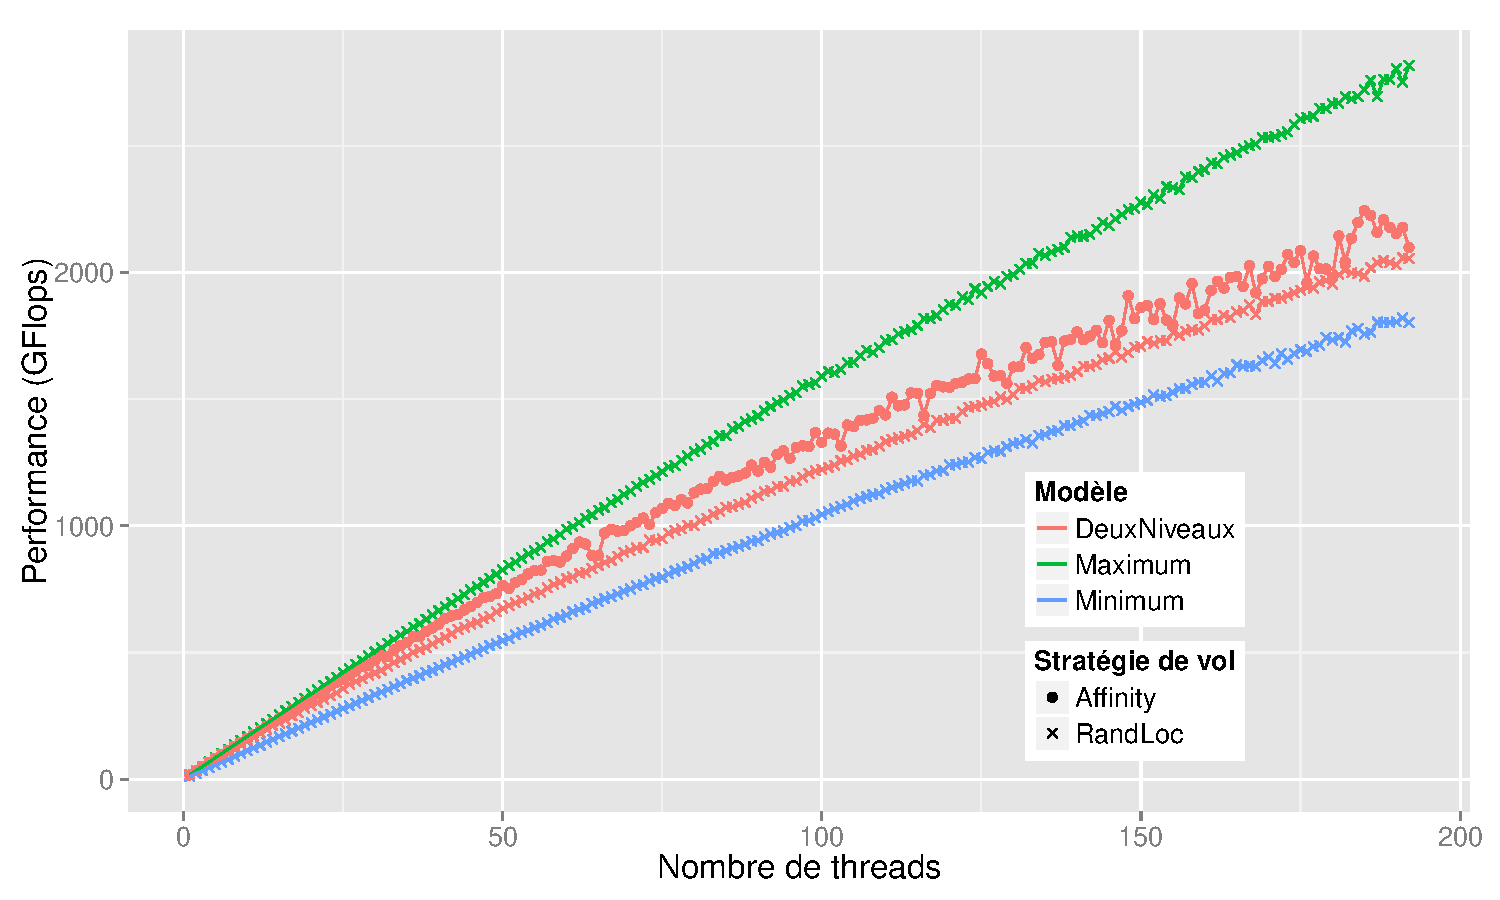
\includegraphics[width=\textwidth]{simu_min_max_affinity_idchire}
  \caption{Comparaison des différents modèles et stratégies, basés sur les références d'idchire. Taille de bloc~: 512, taille de matrice~: 32768}\label{fig:simu:modeles:idchire}
\end{figure}


Les premières observations à faire sur cette figure sont plutôt positives~: les performances affichées semblent réalistes, le modèle \emph{Affinity} est correctement encadré par les modèles \emph{Minimum} et \emph{Maximum}, et au sein du modèle \emph{Affinity}, il y a bien une différence claire entre un vol de travail <<naïf>> --- \emph{RandLoc} --- et un vol de travail hiérarchique et sensible à l'affinité --- \emph{Affinity}.

\begin{table}[h!]
\def\arraystretch{1.5}
\centering
\begin{tabular}{|c||c|c|c|c|}\hline
  \multirow{2}{*}{Stratégie} & \multicolumn{2}{c|}{Lectures} & \multicolumn{2}{c|}{Écritures} \\ \cline{2-5}
    & Locales & Distantes & Locales & Distantes \\
  \hline
  \emph{RandLoc} & 4 380 & 117 066 & 1902 & 43 858 \\
  \hline
  \emph{Affinity} & 15 343 & 88 045 & 22 556 & 23 204 \\
  \hline
\end{tabular}
\caption{Nombre de lectures et écritures de blocs locaux ou distants en fonction de la stratégie de vol}\label{tab:simu:acces-blocs-idchire}
\end{table}
\begin{todo}
Note : cumul des lectures dans la table différent puisque cache infini : si lecture une fois sur le nœud, c'est gratos après si la version change pas.
\end{todo}

Cela est confirmé en regardant le nombre de lectures et écritures locales ou distantes, rapportées dans le tableau~\ref{tab:simu:acces-blocs-idchire}.
Ce tableau montre que le nombre d'accès distants est significativement diminué par l'utilisation d'une stratégie de vol de travail sensible à l'affinité~: le nombre d'écritures distantes est réduit de moitié, tandis que le nombre de lectures distantes est réduit d'environ 25\%.


Ces figures sont bien sur issues de simulation~; que valent elles en comparaison aux chiffres obtenus à travers les expériences ?

\begin{figure}[t!]
  \centering
  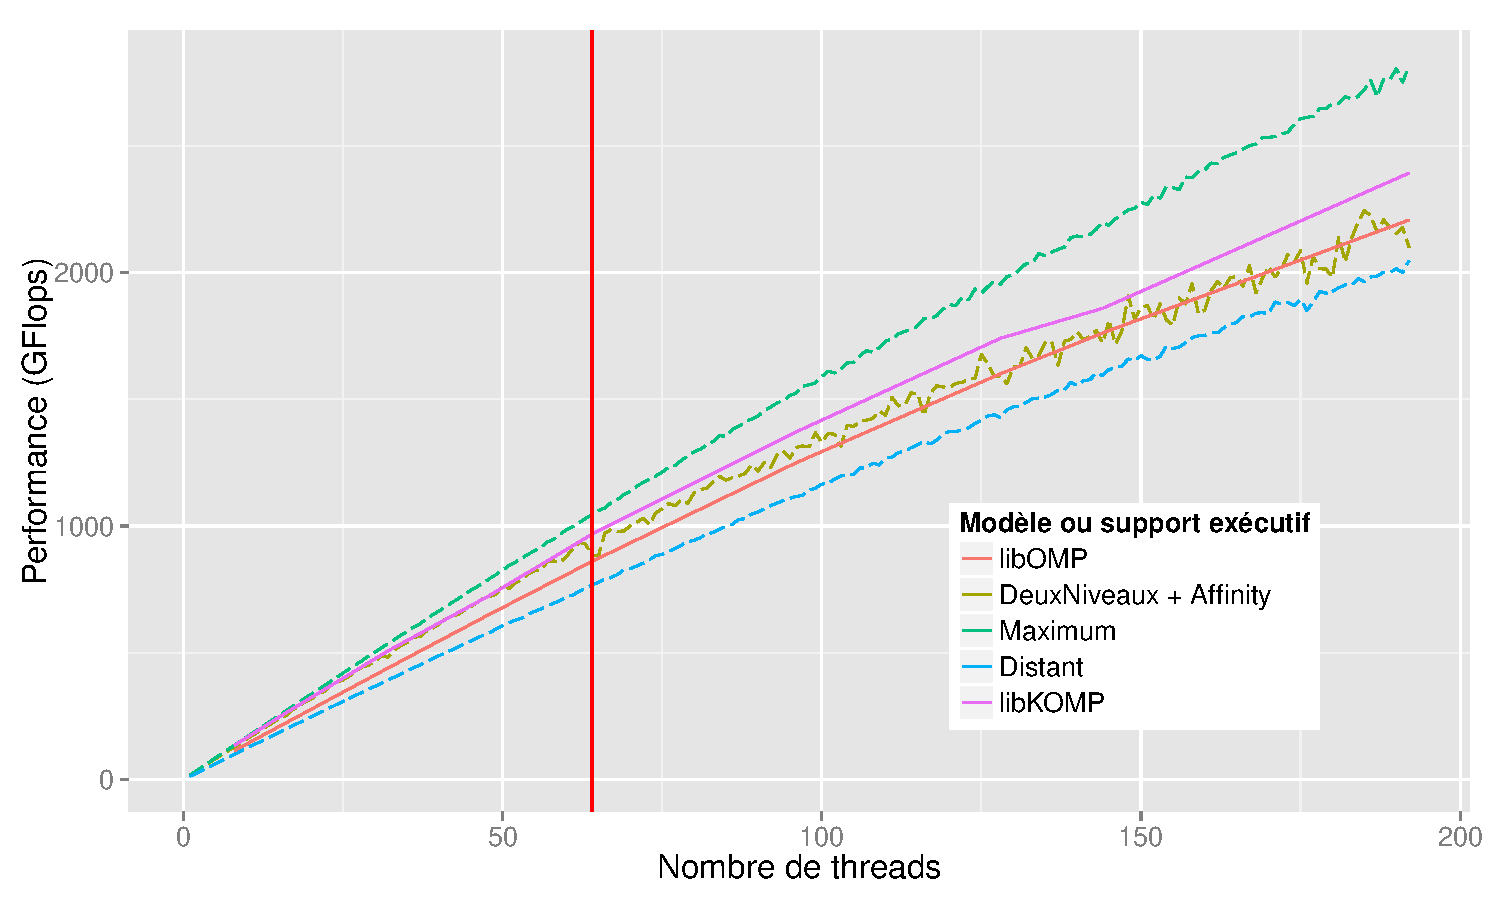
\includegraphics[width=\textwidth]{simu_affinity_runtime_idchire}
  \caption{Comparaison des certains modèles aux supports exécutifs sur idchire, pour une taille de matrice de 32768 et une taille de bloc de 512}\label{fig:simu:modeles-vs-runtime:idchire}
\end{figure}
\begin{figure}[h!]
  \centering
  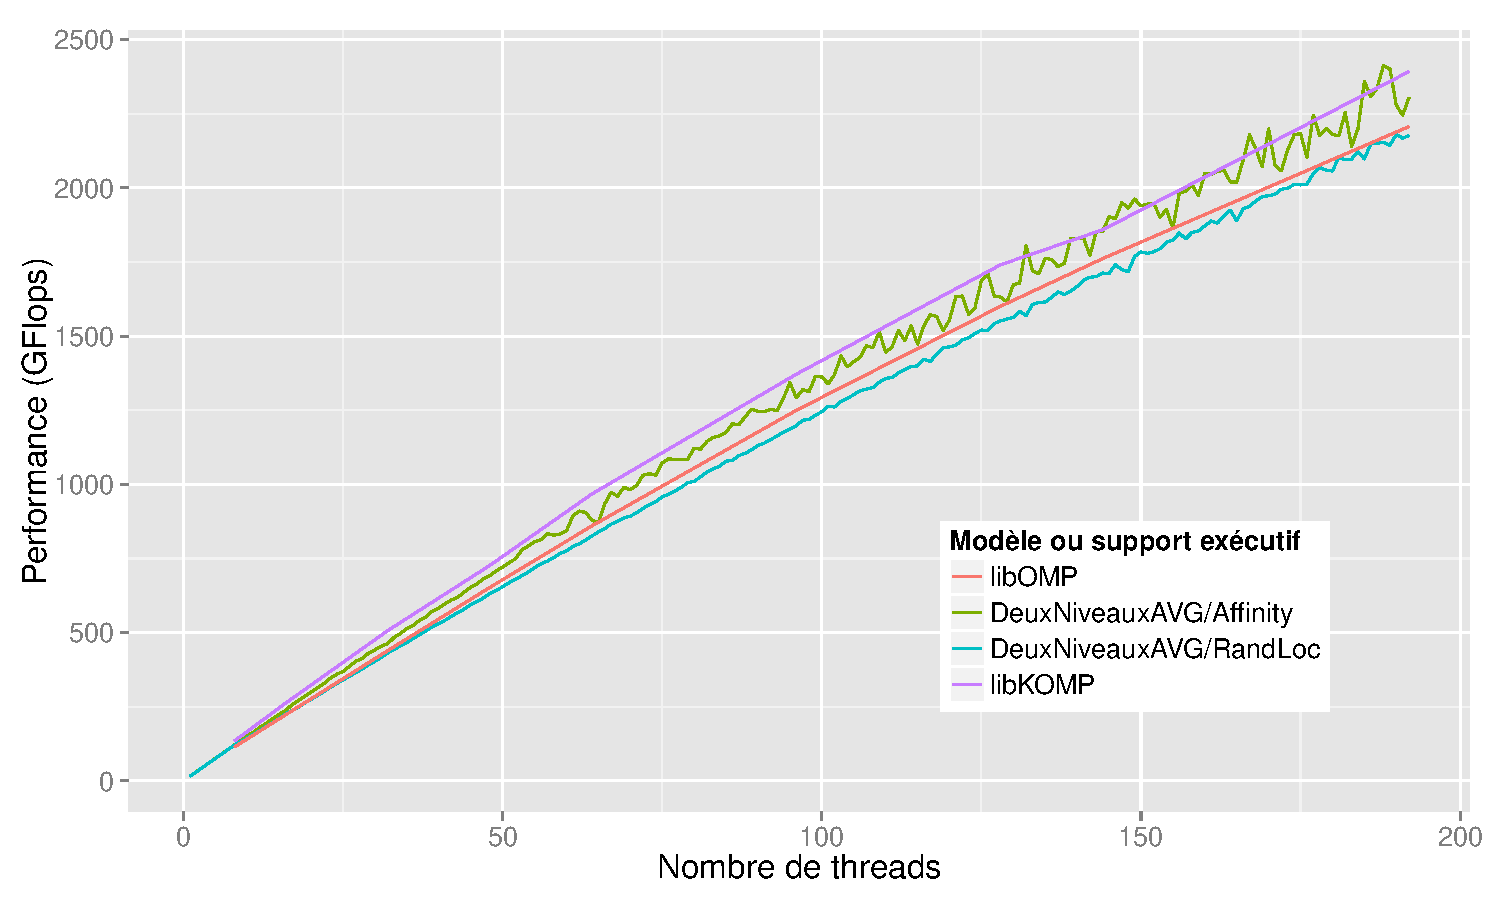
\includegraphics[width=\textwidth]{simu_affinity_avg_runtime_idchire}
  \caption{Comparaison du modèle \emph{AffinityAVG} aux supports exécutifs sur idchire, pour une taille de matrice de 32768 et une taille de bloc de 512}\label{fig:simu:affinityavg-vs-runtime:idchire}
\end{figure}


La figure~\ref{fig:simu:modeles-vs-runtime:idchire} compare les modèles \emph{Minimum} (avec vol aléatoire) et \emph{Affinity} (avec vol hiérarchique) aux supports exécutifs libOMP et libKOMP. libGOMP a été omis pour ne pas surcharger la figure, et parce que son comportement suit celui de libOMP.
Comme on peut le constater, les performances des deux supports exécutifs sont effectivement supérieures au minimum simulé. En revanche les performances simulées de l'affinité semblent faibles compte tenu des performances réelles.

Cette différence pourrait sembler étonnante, mais pourrait être en partie expliquée par le fait que les performances de référence ont été obtenues lorsque les données étaient soit \textit{toutes} locales ou \textit{toutes} distantes.
Alors que dans la réalité il peut évidemment y avoir plusieurs autres cas quand plusieurs blocs sont en paramètre des noyaux.
Cela donnerait donc une version <<minimum>> des performances plus pessimistes que la réalité.

Nous avons essayé de prendre la moyenne globale des performances de chaque noyau comme référence, sous le modèle \emph{AffinityAVG}.
Les résultats obtenus sont présentés sur la figure~\ref{fig:simu:affinityavg-vs-runtime:idchire}.

La simulation des deux heuristiques semblent adhérer un peu mieux à la réalité, bien qu'il semble possible de gagner encore en précision.

Ces travaux étant en cours, plusieurs pistes d'amélioration sont envisagées, et sont décrites dans la section~\ref{sec:simulation:next}.


Les résultats obtenus sur les cas favorable à l'utilisation de l'affinité sont assez encourageants.
Nous avons également appliqué la simulation sur des tailles de bloc plus petites, typiquement pour une taille de matrice de 8192 avec des blocs de 256.

\begin{figure}[h!]
  \centering
  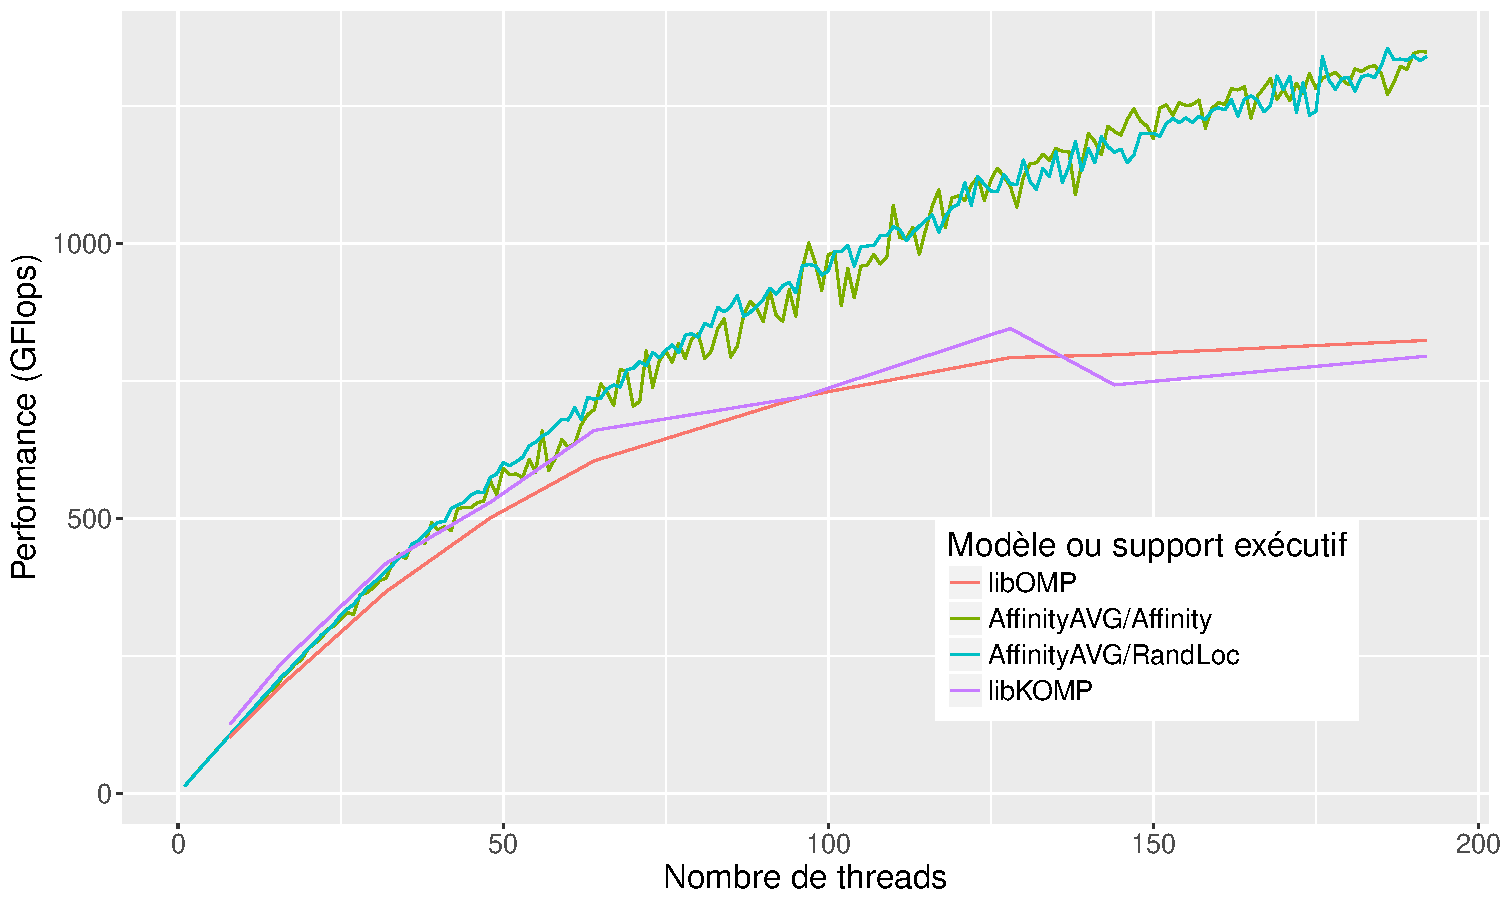
\includegraphics[width=\textwidth]{simu_affinity_8k_runtime_idchire}
  \caption{Comparaison du modèle \emph{AffinityAVG} aux supports exécutifs sur idchire, pour une taille de matrice de 8192 et une taille de bloc de 256}\label{fig:simu:affinityavg-8k-vs-runtime:idchire}
\end{figure}

Les résultats obtenus sont présentés sur la figure~\ref{fig:simu:affinityavg-8k-vs-runtime:idchire}.
Comme on a pu le constater sur les expériences réelles, la simulation ne montre également aucune différence de performances avec ou sans l'utilisation de l'affinité.

En revanche les performances des deux supports exécutifs sont assez loin de celles a priori atteignables !
Le nombre de tâches dans une telle configuration peut vite limiter le parallélisme exposé, ce qui va donc entrainer une augmentation importante du nombre de requêtes de vol émises par les threads inactifs.

Ces requêtes ne sont pas modélisées dans le simulateur, et peuvent générer du trafic sur les bus mémoires~: donc non seulement les threads ne participent plus activement à l'exécution du programme, mais en plus ils peuvent dégrader les performances des threads actifs.
Cela peut expliquer en grande partie la différence entre la simulation et la réalité, et pourrait être une piste d'amélioration du modèle.


\section{Application d'un ordonnancement théorique}\label{sec:simulation:theorie}

ref model:

\cite{Pan2014}, Modeling cache coherence misses on multicores

\cite{Stanisic2016}, Fast and Accurate Simulation of Multithreaded Sparse Linear Algebra Solvers

\begin{todo}
GRAPHE : courbes Julien sur Cholesky sélectionnés

+mettre la section dans un endroit approprié, probablement après la description du modèle histoire de dire "ça c'est ce qu'on peut faire au mieux".
\end{todo}

\section{Discussions et améliorations possibles}\label{sec:simulation:next}

Nos travaux sur la simulation sont très récent et encore en cours de développement.
Afin de généraliser la portée du simulateur et améliorer sa précision, nous évoquons ici les différentes pistes en cours d'étude.

\subsection{Modélisation du cache L3}

La version actuelle du simulateur inclue un cache par cœur de taille infinie.
Ce cache est modélisé comme une liste de blocs, dans une \emph{version} particulière.
À chaque écriture du bloc, la version du bloc est incrémentée.
Si une tâche effectue une lecture de ce bloc et que sa version correspond à la version du cache, alors la lecture ne coûte rien, sinon le cout de lecture est demandé au modèle.

Comme indiqué dans les sections précédentes, les modèles envisagés pour l'instant se basent uniquement sur le cout global d'une tâche, plutôt que sur des actions séparées.

L'une des améliorations nécessaires pour augmenter la précision du modèle serait l'introduction d'un cache partagé entre les cœurs d'un même nœud, disposant d'une capacité définie par le modèle, et implémentant une politique d'éviction relativement proche de celle utilisée par le matériel~: \emph{LRU}.

\subsection{Modélisation de la bande passante}

Le chapitre~\ref{chap:contrib:characterization} nous a permis d'étudier en détail le comportement de nos deux machines d'expériences.
Les figures~\ref{fig:contribs:machines:idchire:saturation} et~\ref{fig:contribs:machines:idchire:saturation-output} permettent de conclure par exemple que la bande passante d'idchire se comporte d'une manière assez proche d'un modèle \emph{roofline}, où elle augmente linéairement avant d'atteindre un <<plafond>>.

L'objectif serait donc d'introduire un coût d'accès aux blocs mémoires suivant ce modèle.

\subsection{Modélisation des surcouts d'ordonnancement}

La figure~\ref{fig:simu:affinityavg-8k-vs-runtime:idchire} l'a montré, le simulateur manque d'un moyen de modéliser les coûts liés aux fonctions d'ordonnancement du support exécutif.
Une manière d'aborder cela pourrait être d'associer un très faible coût à chaque requête de vol, et éventuellement de le pondérer par le nombre de threads en train d'effectuer des requêtes, pour modéliser la synchronisation nécessaire.

\subsection{Optimisation de la distribution}

Le simulateur permet d'obtenir des informations précises sur la distribution de données et son impact sur les accès locaux et distants.
Comme on l'a vu dans le tableau~\ref{tab:simu:acces-blocs-idchire}, le vol de travail respectant l'affinité permet de réduire considérablement les accès distants.
Il devrait donc être possible d'utiliser le simulateur pour automatiquement trouver la <<meilleure>> distribution de données (c'est à dire celle qui minimise les accès distants), en se basant sur une distribution cyclique et en introduisant des paramètres tels que le premier nœud considéré, le nombre de blocs alloués en même temps, et le pas lors du parcours des nœuds.

\part{Perspectives et conclusion}

\chapter{Vers une amélioration possible du support exécutif à travers la simulation}\label{chap:simulation}
\chaptertoc

Le chapitre~\ref{chap:contrib:characterization} a montré qu'il était possible de caractériser précisément à la fois les machines et les parties critiques d'application.
Cela a pu confirmer et chiffrer l'importance de la localité des données sur les architectures NUMA.
Le chapitre~\ref{chap:contrib:openmp} a montré comment il était possible d'étendre un modèle de programmation et les supports exécutifs pour mieux prendre en compte la localité des données, et globalement améliorer l'ordonnancement de l'application.

À partir de là, certaines questions peuvent se poser~:
\begin{itemize}
  \item Compte tenu des caractéristiques de l'application et des machines, peut on faire mieux ? Et si oui~:
  \item Quelle marge reste-t'il à gagner par rapport à aux ordonnancements théorique connus ?
  \item Quelles caractéristiques faudrait il prendre en compte ?
\end{itemize}

Le coût en temps d'un développement de nouvelles analyses ou stratégies dans les compilateurs et supports exécutifs peut être important. Ainsi avant de se lancer il serait préférable de connaître le potentiel des améliorations.
Nous avons donc développé un simulateur, dans le but de pouvoir apporter une réponse aux questions ci-dessus, sans pour autant impliquer de lourds développements logiciel.

Ce chapitre est organisé de la façon suivante~: la section~\ref{sec:simulation:archi} décrit l'architecture générale du simulateur.
La section~\ref{sec:simulation:modeles} fait un point sur les différents modèles envisagés, et la section~\ref{sec:simulation:resultats} montre des résultats préliminaires obtenus avec ces modèles, en apportant des premières pistes de réponses aux questions posées.
Enfin la section~\ref{sec:simulation:next} décrit quels améliorations du simulateur seraient possible pour améliorer son réalisme.

TODO rajouter introduction section Julien si possible


\section{Fonctionnement du simulateur}\label{sec:simulation:archi}

Le simulateur implémente un certain nombre de concepts que nous avons déjà abordés, détaillés ci-après.


\paragraph{Données~:} elles sont représentés comme des blocs de tailles fixes, qui sont associés à un cœur lors de leur création (pour simuler la politique \emph{first-touch} du système d'exploitation).

\paragraph{Tâches~:} elles sont représentées de manière similaire à ce qui se fait dans les supports exécutifs.
Chaque tâche est composée d'une série d'actions séquentielles, pouvant être de trois types différents~:
\begin{itemize}
  \item \emph{READ}~: lecture d'un bloc de données
  \item \emph{WRITE}~: écriture d'un bloc de données
  \item \emph{COMPUTE}~: calcul avec un certain nombre d'instructions.
\end{itemize}

De plus des dépendances entre tâches peuvent être ajoutées en attachant un ensemble de prédécesseurs à une tâche donnée.

\paragraph{Topologie~:}
De manière similaire à ce que nous avons utilisé lors de nos travaux, nous avons considéré ici deux niveaux de hiérarchie, avec une file de tâche prêtes par cœur, et une file de tâche prêtes par nœud.

\paragraph{Ordonnancement~:}
L'objectif était de simuler le comportement d'un support exécutif similaire à ceux que nous avons utilisé dans le chapitre~\ref{chap:contrib:openmp}, nous avons donc basé l'ordonnancement au sein du simulateur sur du vol de travail.
Le moteur d'exécution repose sur deux fonction \emph{steal} et \emph{push}, devant implémenter les processus de vol et de placement d'une tâche, respectivement.
Pour le besoin des premières comparaisons, nous avons implémenté deux heuristiques différentes, similaires à celles utilisées dans les résultats de la section~\ref{sec:contribs:perf_eval}~:
\begin{itemize}
  \item \emph{RandLoc}~: elle effectue du vol de travail aléatoire de base et un placement des tâches prêtes localement~; elle est équivalente à la combinaison de stratégies \emph{sRand/pLoc} décrites dans la section~\ref{sec:openmp:runtime:select}.
  \item \emph{Affinity}~: elle effectue un vol de travail hiérarchique et un placement des tâches conformément à l'affinité des données~; elle est équivalente à la combinaison \emph{sNumaProc/pNumaWLoc} décrites dans la section~\ref{sec:openmp:runtime:select}.
\end{itemize}


\paragraph{Modèle~:}
Un modèle fourni des informations cruciales~: il défini la topologie de la machine (nombre de cœurs, de nœuds, ainsi que les associations cœur/nœud), il défini également le coût de chaque opération (exprimé en secondes) en fonction de son type et du type de la tâche effectuant l'opération.


\section{Modèles envisagés}\label{sec:simulation:modeles}

Nous avons choisi de commencer à étudier l'application qui nous a servi de cas d'étude pour le chapitre~\ref{chap:contrib:characterization}~: Cholesky.
Les données récoltés à l'aide de \outil nous ont permises de comprendre précisément le comportement de chacun des quatre noyaux impliqués dans la factorisation de Cholesky.
Nous avons donc implémenté un Cholesky similaire dans le simulateur, et défini plusieurs modèles afin d'évaluer le simulateur et éventuellement les bornes de l'application en terme de performances.

Comme les données récoltées sur les noyaux inclus la totalité des actions des tâches (lecture, calcul, et écriture), nous avons donc dans un premier utilisé un modèle simplifié, où la quantité de données en lecture et écriture est ignorée, mais ou la partie \emph{COMPUTE} inclue ces accès, et dépend du placement du bloc de données sur la machine simulée.

\begin{table}[t!]
\def\arraystretch{1.5}
\centering
\begin{tabular}{|c||c|c|c|}\hline
  \multirow{2}{*}{Noyau} & \multirow{2}{*}{\makecell{Nombre d'exécution concurrentes\\(threads)}} & \multicolumn{2}{c|}{Performance (GFLOPS)} \\ \cline{3-4}
    & & Données locales & Données distantes \\ \hline
  \multirow{2}{*}{\potrf}
    & 1 & 11.66 & 11.66 \\ \cline{2-4}
    & 192 & 9.30 & 8.81 \\ \cline{2-4}
  \hline
  \multirow{2}{*}{\gemm}
    & 1 & 16.92 & 16.92 \\ \cline{2-4}
    & 192 & 14.45 & 12.82 \\ \cline{2-4}
  \hline
\end{tabular}
\caption{Tableau illustrant les performances (en GFLOPS) de certains noyaux sur des matrices de taille 512, sur idchire}\label{tab:simu:perf-kernels-idchire}
\end{table}

Afin de pouvoir illustrer les différents modèle que nous avons testé, le tableau~\ref{tab:simu:perf-kernels-idchire} regroupe quelques exemples de performance de référence pour certains noyaux, pour une taille de matrice de 512, en fonction de la charge de la machine (comme décrit dans la section~\ref{sec:contribs:apps:cholesky:scenario}) et du type d'accès.

Cet extrait de performances permet de montrer que si la localité des données n'a pas d'impact pour un unique thread, en pleine charge la différence de performance est significative.

Nous avons donc dégagé plusieurs modèles, décrit ci-dessous.

\paragraph{Modèle "Minimum"~:} ce modèle a pour but d'estimer la performance minimum que l'on est en droit d'attendre d'un support exécutif implémentant une stratégie de vol de travail naïve.
Pour se faire, nous avons considéré seulement les performances minimales de chacun des noyaux pour le coût de chaque tâche (il est généralement atteint pour une charge équivalente au maximum de cœur, avec des accès aux données distants), et ceci quelque soit le vrai type d'accès au cours de la simulation.

\paragraph{Modèle "Maximum"~:} à l'inverse l'objectif de ce modèle est de donner une borne supérieure pour les performances du support exécutif.
Nous avons donc considéré seulement les performances maximales de chacun des noyaux pour le coût de chaque tâche, et ceci quelque soit le vrai type d'accès au cours de la simulation.

\paragraph{Modèle "Affinity"~:} l'objectif de ce modèle est d'essayer de simuler au plus près le comportement des noyaux.
La simulation étant lancée sur un nombre de cœurs connus, nous avons chargé les performances de référence des noyaux correspondant à la charge de la machine simulée.
Lors de la simulation nous déterminons si les accès de la tâche sont locaux ou distant, et le coût de la tâche correspondante est utilisé.




\section{Résultats préliminaires}\label{sec:simulation:resultats}


Nous avons commencé par comparer les modèles entre eux.
Pour ce faire nous avons choisi un cas réel ou l'affinité avait un impact significatif~: une taille de bloc de 512 pour une taille de matrice de 32768, avec des blocs de données répartis de manière cyclique sur la machine.
Les résultats des simulations avec les différents modèles sont montrés sur la figure~\ref{fig:simu:modeles:idchire}.

\begin{figure}[h!]
  \centering
  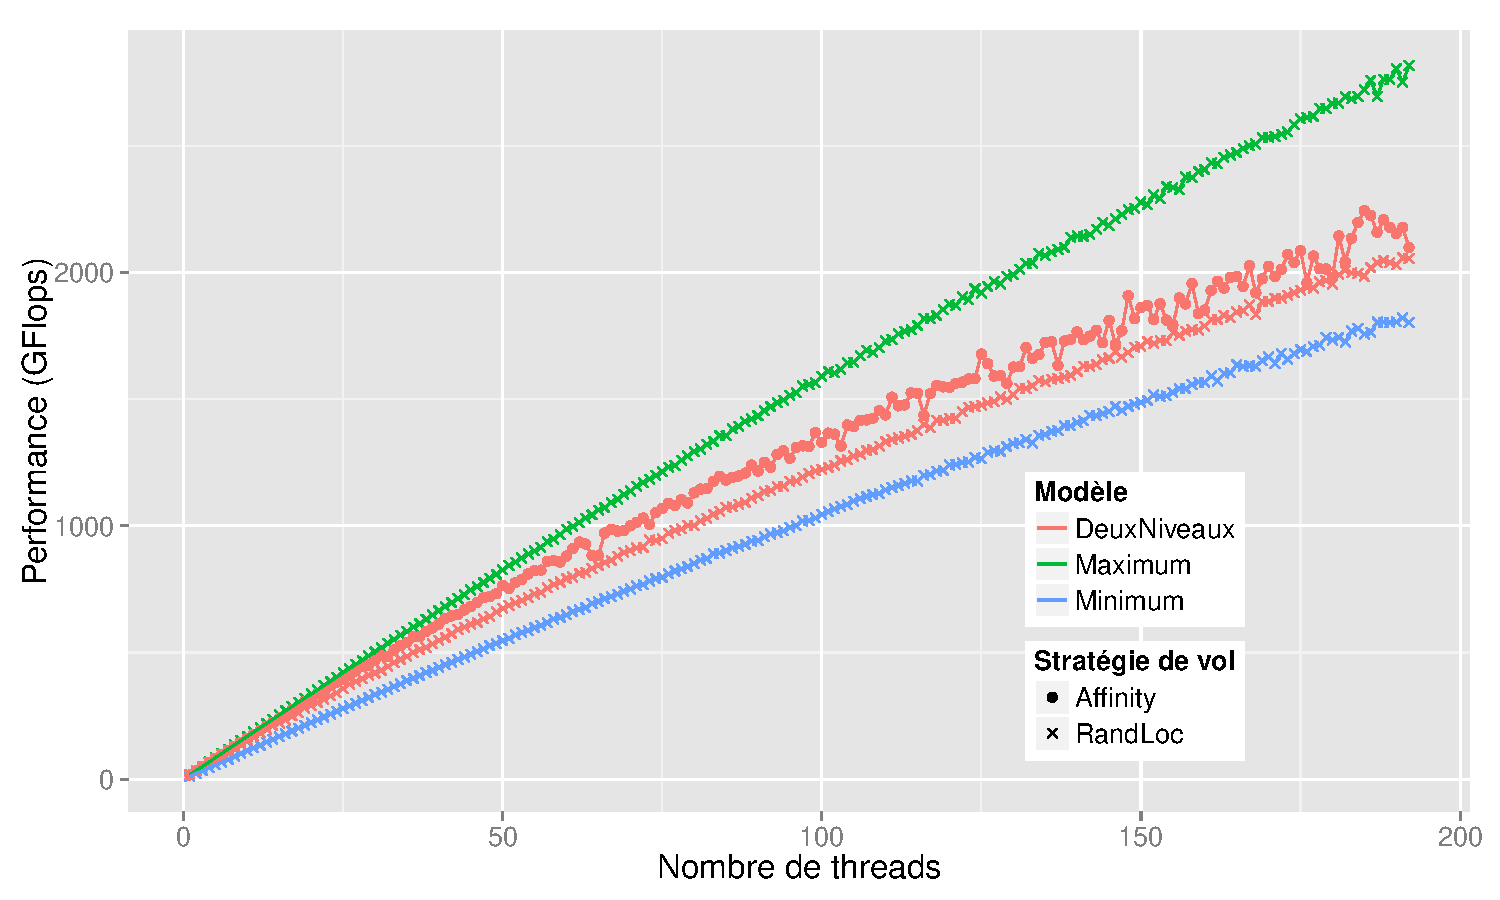
\includegraphics[width=\textwidth]{simu_min_max_affinity_idchire}
  \caption{Comparaison des différents modèles et stratégies, basés sur les références d'idchire. Taille de bloc~: 512, taille de matrice~: 32768}\label{fig:simu:modeles:idchire}
\end{figure}


Les premières observations à faire sur cette figure sont plutôt positives~: les performances affichées semblent réalistes, le modèle \emph{Affinity} est correctement encadré par les modèles \emph{Minimum} et \emph{Maximum}, et au sein du modèle \emph{Affinity}, il y a bien une différence claire entre un vol de travail <<naïf>> --- \emph{RandLoc} --- et un vol de travail hiérarchique et sensible à l'affinité --- \emph{Affinity}.

\begin{table}[h!]
\def\arraystretch{1.5}
\centering
\begin{tabular}{|c||c|c|c|c|}\hline
  \multirow{2}{*}{Stratégie} & \multicolumn{2}{c|}{Lectures} & \multicolumn{2}{c|}{Écritures} \\ \cline{2-5}
    & Locales & Distantes & Locales & Distantes \\
  \hline
  \emph{RandLoc} & 4 380 & 117 066 & 1902 & 43 858 \\
  \hline
  \emph{Affinity} & 15 343 & 88 045 & 22 556 & 23 204 \\
  \hline
\end{tabular}
\caption{Nombre de lectures et écritures de blocs locaux ou distants en fonction de la stratégie de vol}\label{tab:simu:acces-blocs-idchire}
\end{table}
\begin{todo}
Note : cumul des lectures dans la table différent puisque cache infini : si lecture une fois sur le nœud, c'est gratos après si la version change pas.
\end{todo}

Cela est confirmé en regardant le nombre de lectures et écritures locales ou distantes, rapportées dans le tableau~\ref{tab:simu:acces-blocs-idchire}.
Ce tableau montre que le nombre d'accès distants est significativement diminué par l'utilisation d'une stratégie de vol de travail sensible à l'affinité~: le nombre d'écritures distantes est réduit de moitié, tandis que le nombre de lectures distantes est réduit d'environ 25\%.


Ces figures sont bien sur issues de simulation~; que valent elles en comparaison aux chiffres obtenus à travers les expériences ?

\begin{figure}[t!]
  \centering
  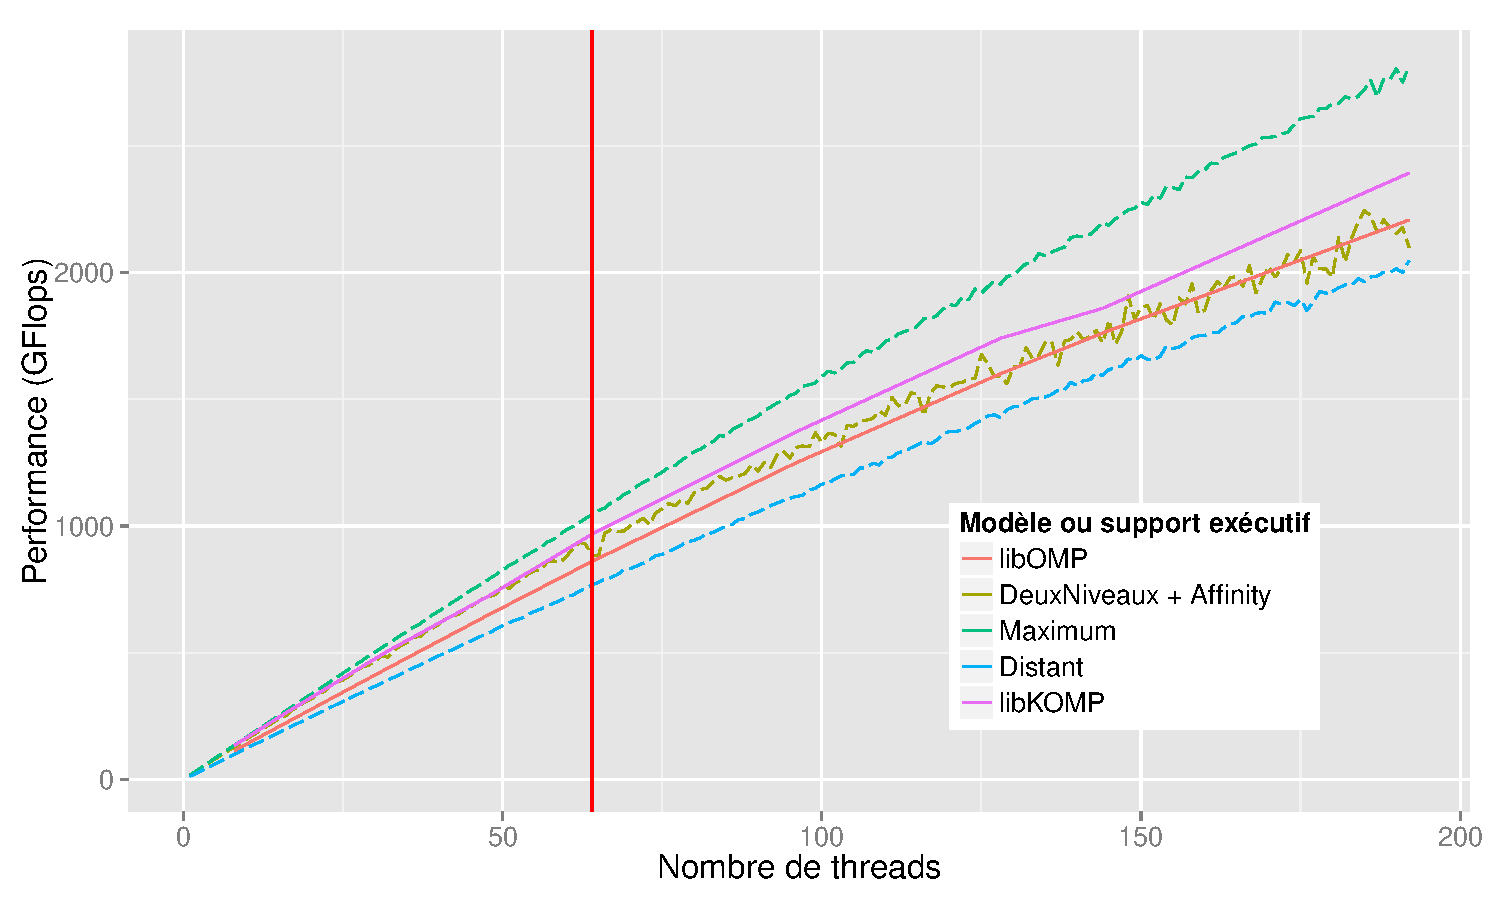
\includegraphics[width=\textwidth]{simu_affinity_runtime_idchire}
  \caption{Comparaison des certains modèles aux supports exécutifs sur idchire, pour une taille de matrice de 32768 et une taille de bloc de 512}\label{fig:simu:modeles-vs-runtime:idchire}
\end{figure}
\begin{figure}[h!]
  \centering
  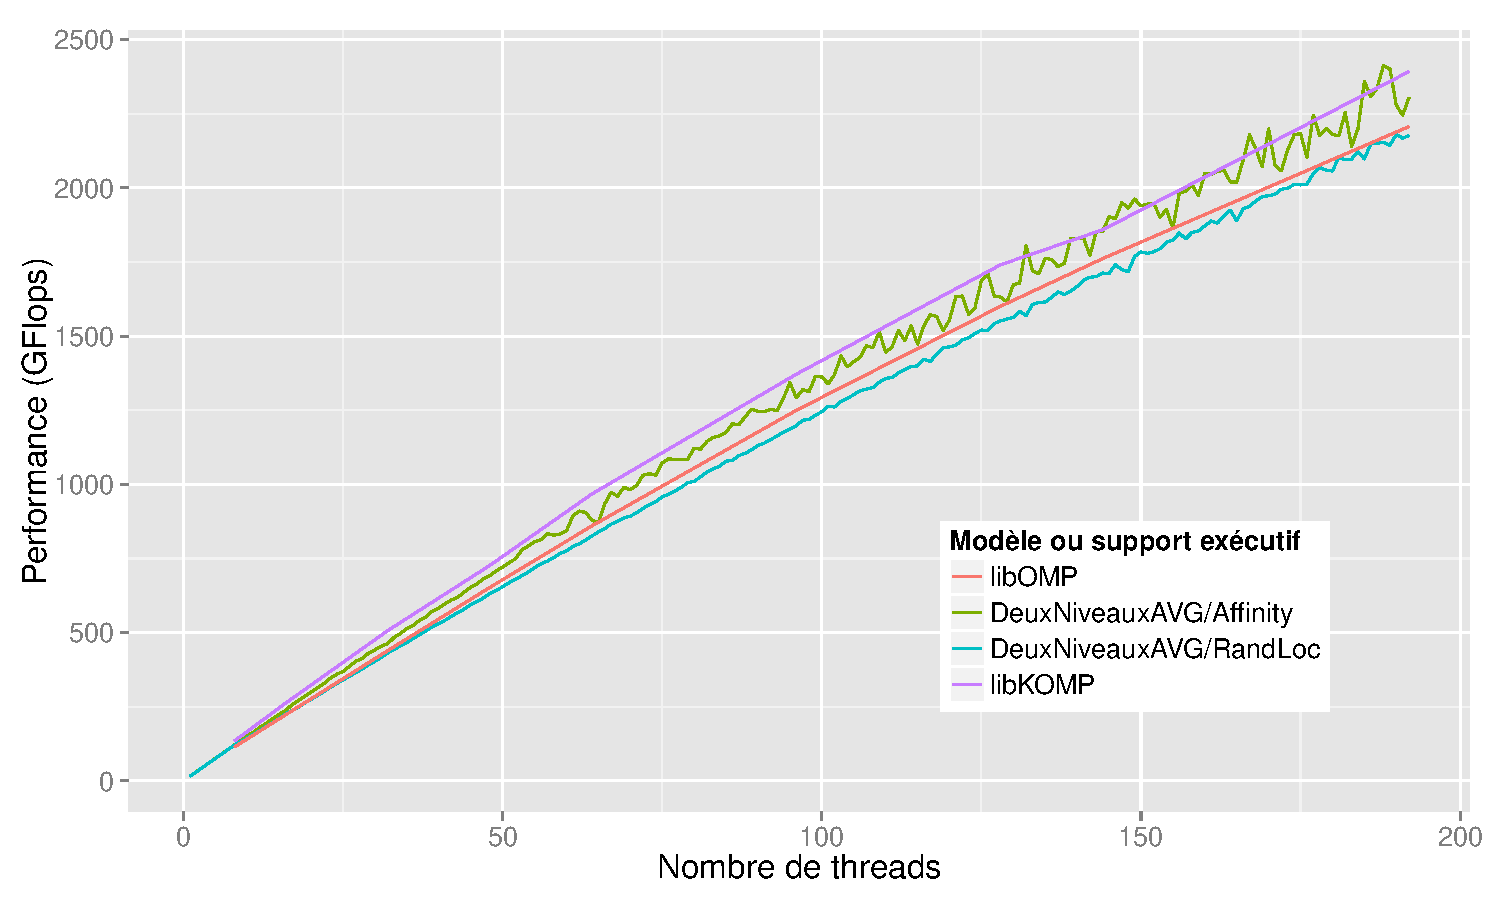
\includegraphics[width=\textwidth]{simu_affinity_avg_runtime_idchire}
  \caption{Comparaison du modèle \emph{AffinityAVG} aux supports exécutifs sur idchire, pour une taille de matrice de 32768 et une taille de bloc de 512}\label{fig:simu:affinityavg-vs-runtime:idchire}
\end{figure}


La figure~\ref{fig:simu:modeles-vs-runtime:idchire} compare les modèles \emph{Minimum} (avec vol aléatoire) et \emph{Affinity} (avec vol hiérarchique) aux supports exécutifs libOMP et libKOMP. libGOMP a été omis pour ne pas surcharger la figure, et parce que son comportement suit celui de libOMP.
Comme on peut le constater, les performances des deux supports exécutifs sont effectivement supérieures au minimum simulé. En revanche les performances simulées de l'affinité semblent faibles compte tenu des performances réelles.

Cette différence pourrait sembler étonnante, mais pourrait être en partie expliquée par le fait que les performances de référence ont été obtenues lorsque les données étaient soit \textit{toutes} locales ou \textit{toutes} distantes.
Alors que dans la réalité il peut évidemment y avoir plusieurs autres cas quand plusieurs blocs sont en paramètre des noyaux.
Cela donnerait donc une version <<minimum>> des performances plus pessimistes que la réalité.

Nous avons essayé de prendre la moyenne globale des performances de chaque noyau comme référence, sous le modèle \emph{AffinityAVG}.
Les résultats obtenus sont présentés sur la figure~\ref{fig:simu:affinityavg-vs-runtime:idchire}.

La simulation des deux heuristiques semblent adhérer un peu mieux à la réalité, bien qu'il semble possible de gagner encore en précision.

Ces travaux étant en cours, plusieurs pistes d'amélioration sont envisagées, et sont décrites dans la section~\ref{sec:simulation:next}.


Les résultats obtenus sur les cas favorable à l'utilisation de l'affinité sont assez encourageants.
Nous avons également appliqué la simulation sur des tailles de bloc plus petites, typiquement pour une taille de matrice de 8192 avec des blocs de 256.

\begin{figure}[h!]
  \centering
  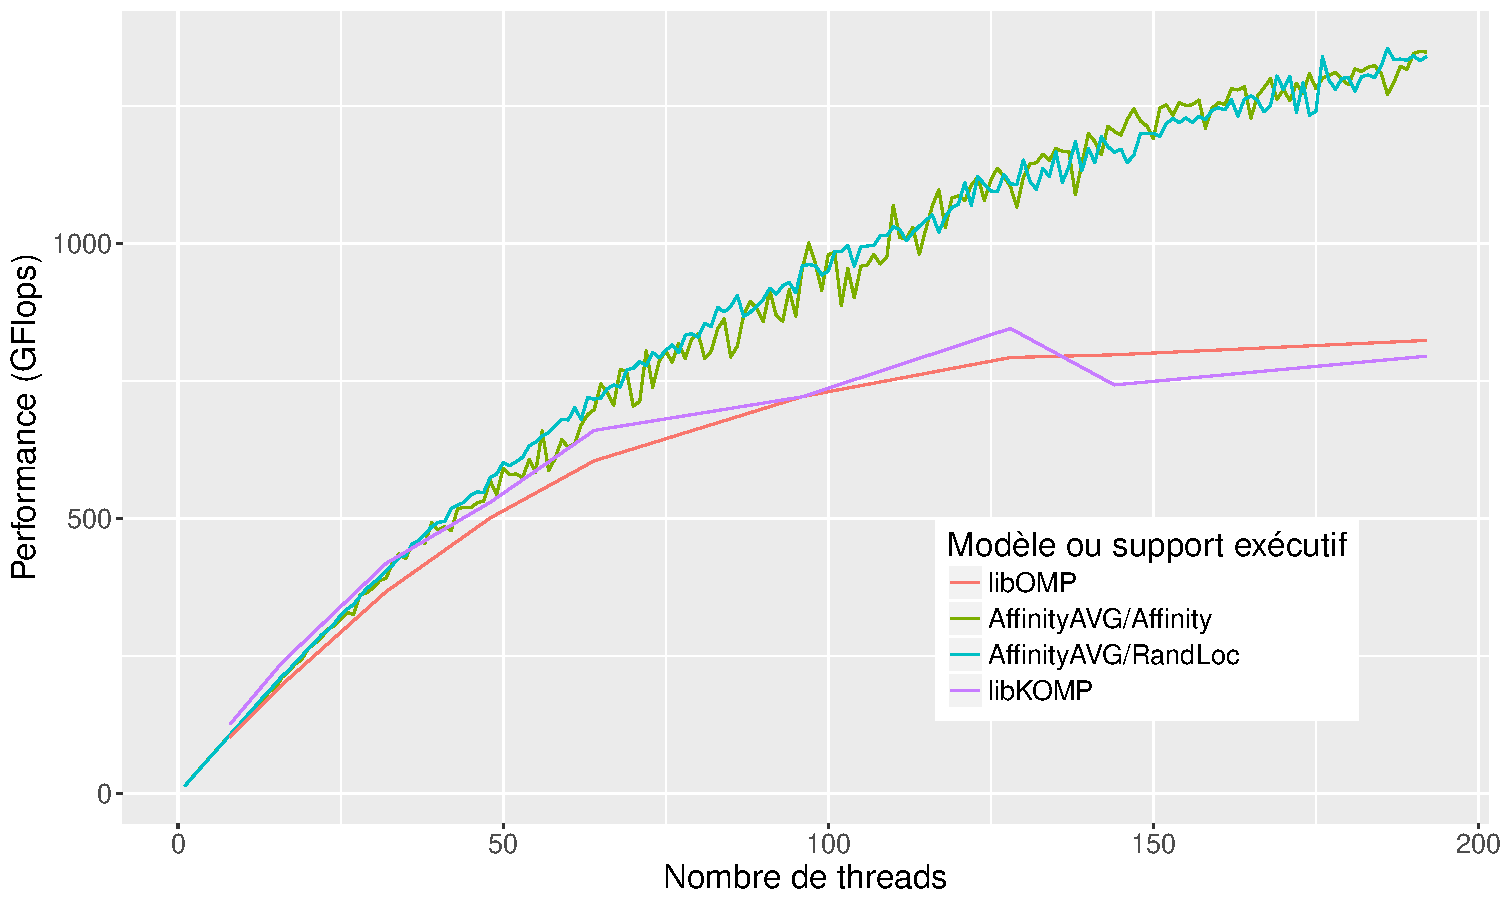
\includegraphics[width=\textwidth]{simu_affinity_8k_runtime_idchire}
  \caption{Comparaison du modèle \emph{AffinityAVG} aux supports exécutifs sur idchire, pour une taille de matrice de 8192 et une taille de bloc de 256}\label{fig:simu:affinityavg-8k-vs-runtime:idchire}
\end{figure}

Les résultats obtenus sont présentés sur la figure~\ref{fig:simu:affinityavg-8k-vs-runtime:idchire}.
Comme on a pu le constater sur les expériences réelles, la simulation ne montre également aucune différence de performances avec ou sans l'utilisation de l'affinité.

En revanche les performances des deux supports exécutifs sont assez loin de celles a priori atteignables !
Le nombre de tâches dans une telle configuration peut vite limiter le parallélisme exposé, ce qui va donc entrainer une augmentation importante du nombre de requêtes de vol émises par les threads inactifs.

Ces requêtes ne sont pas modélisées dans le simulateur, et peuvent générer du trafic sur les bus mémoires~: donc non seulement les threads ne participent plus activement à l'exécution du programme, mais en plus ils peuvent dégrader les performances des threads actifs.
Cela peut expliquer en grande partie la différence entre la simulation et la réalité, et pourrait être une piste d'amélioration du modèle.


\section{Application d'un ordonnancement théorique}\label{sec:simulation:theorie}

ref model:

\cite{Pan2014}, Modeling cache coherence misses on multicores

\cite{Stanisic2016}, Fast and Accurate Simulation of Multithreaded Sparse Linear Algebra Solvers

\begin{todo}
GRAPHE : courbes Julien sur Cholesky sélectionnés

+mettre la section dans un endroit approprié, probablement après la description du modèle histoire de dire "ça c'est ce qu'on peut faire au mieux".
\end{todo}

\section{Discussions et améliorations possibles}\label{sec:simulation:next}

Nos travaux sur la simulation sont très récent et encore en cours de développement.
Afin de généraliser la portée du simulateur et améliorer sa précision, nous évoquons ici les différentes pistes en cours d'étude.

\subsection{Modélisation du cache L3}

La version actuelle du simulateur inclue un cache par cœur de taille infinie.
Ce cache est modélisé comme une liste de blocs, dans une \emph{version} particulière.
À chaque écriture du bloc, la version du bloc est incrémentée.
Si une tâche effectue une lecture de ce bloc et que sa version correspond à la version du cache, alors la lecture ne coûte rien, sinon le cout de lecture est demandé au modèle.

Comme indiqué dans les sections précédentes, les modèles envisagés pour l'instant se basent uniquement sur le cout global d'une tâche, plutôt que sur des actions séparées.

L'une des améliorations nécessaires pour augmenter la précision du modèle serait l'introduction d'un cache partagé entre les cœurs d'un même nœud, disposant d'une capacité définie par le modèle, et implémentant une politique d'éviction relativement proche de celle utilisée par le matériel~: \emph{LRU}.

\subsection{Modélisation de la bande passante}

Le chapitre~\ref{chap:contrib:characterization} nous a permis d'étudier en détail le comportement de nos deux machines d'expériences.
Les figures~\ref{fig:contribs:machines:idchire:saturation} et~\ref{fig:contribs:machines:idchire:saturation-output} permettent de conclure par exemple que la bande passante d'idchire se comporte d'une manière assez proche d'un modèle \emph{roofline}, où elle augmente linéairement avant d'atteindre un <<plafond>>.

L'objectif serait donc d'introduire un coût d'accès aux blocs mémoires suivant ce modèle.

\subsection{Modélisation des surcouts d'ordonnancement}

La figure~\ref{fig:simu:affinityavg-8k-vs-runtime:idchire} l'a montré, le simulateur manque d'un moyen de modéliser les coûts liés aux fonctions d'ordonnancement du support exécutif.
Une manière d'aborder cela pourrait être d'associer un très faible coût à chaque requête de vol, et éventuellement de le pondérer par le nombre de threads en train d'effectuer des requêtes, pour modéliser la synchronisation nécessaire.

\subsection{Optimisation de la distribution}

Le simulateur permet d'obtenir des informations précises sur la distribution de données et son impact sur les accès locaux et distants.
Comme on l'a vu dans le tableau~\ref{tab:simu:acces-blocs-idchire}, le vol de travail respectant l'affinité permet de réduire considérablement les accès distants.
Il devrait donc être possible d'utiliser le simulateur pour automatiquement trouver la <<meilleure>> distribution de données (c'est à dire celle qui minimise les accès distants), en se basant sur une distribution cyclique et en introduisant des paramètres tels que le premier nœud considéré, le nombre de blocs alloués en même temps, et le pas lors du parcours des nœuds.

\part{Perspectives et conclusion}

\input{tex/conclusion/simulation}
\input{tex/conclusion/conclusion}



